\pdfoutput=1
\documentclass{l4proj}

\usepackage[UKenglish]{babel}
\usepackage[UKenglish]{isodate}
\PassOptionsToPackage{hyphens}{url}\usepackage[hidelinks]{hyperref}
\usepackage{amsfonts, amsmath, amsthm, graphicx, subcaption, mathtools,
  tikz, cancel}
\usepackage[group-separator={,}]{siunitx}
\usepackage[linesnumbered]{algorithm2e}
\usetikzlibrary{positioning}

\newtheorem{lemma}{Lemma}[chapter]
\newtheorem{proposition}{Proposition}[chapter]
\theoremstyle{definition}
\newtheorem{definition}{Definition}[chapter]
\newtheorem{example}{Example}[chapter]
\theoremstyle{remark}
\newtheorem{remark}{Remark}[chapter]

\DeclareMathOperator{\dom}{dom}
\newcommand{\kprec}[1]{\prescript{}{#1}{\preceq}\ }

\title{Algorithm Selection for Maximum Common Subgraph}
\author{Paulius Dilkas}
%\date{}

\begin{document}
\maketitle

%\begin{abstract} TODO: obviously
%\end{abstract}

\educationalconsent
\tableofcontents

\chapter{Introduction}
\pagenumbering{arabic}

TODO: introduce algorithm selection more formally

The purpose of this project is to create and explore machine learning-based
algorithm \emph{portfolios}, i.e., machine learning models whose main goal is to
provide a mapping, assigning the best-performing algorithm to each problem
instance \cite{DBLP:journals/ai/BischlKKLMFHHLT16, DBLP:journals/ac/Rice76}.

We begin with a definition of a graph suitable for the empirical data described
in Chapter \ref{chapter:problems} and used in Chapter
\ref{chapter:generating_data}.

\begin{definition}
  Let $S$ be a set and $k$ a non-negative integer. Then $[S]^k$ denotes
  the set of \emph{$k$-subsets} of $S$ \cite{subset}, i.e.,
  \[ [S]^k = \{ A \subseteq S : |A| = k \}. \]
\end{definition}

\begin{definition} \label{def:graph}
  An \emph{undirected multigraph} is a pair $(V, E)$, where $V$ is a set of
  vertices and $E$ is a set of edges, together with a map $E \to V \cup [V]^2$,
  which assigns one or two vertices to each edge
  \cite{DBLP:books/daglib/0030488}. If an edge is assigned to a single vertex,
  it is called a \emph{loop}. When several edges map to the same pair of
  vertices, they are referred to as \emph{multiple edges}. 
\end{definition}

For the purposes of this project, we look at two kinds of labelled graphs: those
with vertex labels, and those with both vertex and edge labels. We define them
as follows (the definitions are loosely inspired by \cite{abu-aisheh_2016}):

\begin{definition} \label{def:vertex_label}
  A \emph{(vertex-)labelled graph} is a 3-tuple $G = (V, E, \mu)$, where $V$,
  $E$ are as in Definition \ref{def:graph} and $\mu \colon V \to \{ 0, \dots, N
  - 1 \}$ is a vertex labelling function, for some $N \in \mathbb{N}$.
\end{definition}

\begin{definition} \label{def:edge_label}
  A \emph{fully labelled graph} is a 4-tuple $G = (V, E, \mu, \zeta)$, where the
  first three elements are as in Definition \ref{def:vertex_label} and $\zeta
  \colon E \to \{ 0, \dots, M - 1 \}$ is an edge labelling function, for some $M
  \in \mathbb{N}$.
\end{definition}

Specifically, note that:

\begin{itemize}
\item If a graph is labelled, then all its vertices (and possibly edges) are
  assigned a label.
\item We are only considering finite sets of labels, represented by non-negative
  integers.
\item A vertex-labelled graph is just a special case of a fully labelled graph
  with $M = 1$.
\item An unlabelled graph is just a special case of of a vertex-labelled graph
  with $N = 1$.
\end{itemize}

The last two observations allow us to tailor subsequent definitions to fully
labelled graphs without having to redefine everything for unlabelled and
vertex-labelled graphs as well. When vertex and/or edge labels are immaterial to
a definition, we will omit the labelling function from the full 4-tuple and
denote a graph as just $G = (V, E)$.

We formulate all definitions in terms of undirected multigraphs as some of the
graphs in Chapter \ref{chapter:problems} contain multiple edges and many contain
at least one loop. In the rest of the dissertation, we will use the word
``graph'' to denote undirected multigraphs. Next we adapt some basic graph
theory definitions to work with our definitions of graphs and labelling. As most
definitions in the literature are typically defined for simple graphs with no
labels, the cited sources are heavily adapted to the full generality of graphs
relevant to this dissertation.

\begin{definition}
  Two graphs $G_1 = (V_1, E_1, \mu_1, \zeta_1)$ and $G_2 = (V_2, E_2, \mu_2,
  \zeta_2)$ are said to be \emph{isomorphic} if there are bijections $f \colon
  V_1 \to V_2$, $g \colon E_1 \to E_2$ such that
  \cite{DBLP:journals/jcamd/RaymondW02a}:
  \begin{itemize}
  \item $\forall e \in E_1$, if $e$ maps to some $v \in V_1 \cup [V_1]^2$, then
    $g(e)$ maps to $f(v)$, where $f(v) = \{ f(v_1), f(v_2) \}$ if $v = \{ v_1,
    v_2 \}$ (preserving structure);
  \item $\forall v \in V_1$, $\mu_2(f(v)) = \mu_1(v)$ (preserving vertex labels)
    \cite{DBLP:journals/siamcomp/BabaiES80};
  \item $\forall e \in E_1$, $\zeta_2(g(e)) = \zeta_1(e)$ (preserving edge
    labels).
  \end{itemize}
\end{definition}

\begin{definition}
  Let $f \colon X \to Y$ be a function. Then the \emph{restriction} of $f$ to $A
  \subseteq X$ is a function $f|_A \colon A \to Y$ such that $\forall a \in A$,
  $f|_A(a) = f(a)$ \cite{stoll1979set}.
\end{definition}

\begin{definition} A graph $G_2 = (V_2, E_2, \mu_2, \zeta_2)$ is a
  \emph{subgraph} of graph $G_1 = (V_1, E_1, \mu_1, \zeta_1)$ if
  \cite{DBLP:books/daglib/0030488}:
  \begin{itemize}
  \item $V_2 \subseteq V_1$,
  \item $E_2 \subseteq E_1$ (with the edge-mapping function restricted to
    $E_2$),
  \item $\mu_2 = \mu_1|_{V_2}$,
  \item $\zeta_2 = \zeta_1|_{E_2}$.
  \end{itemize}
\end{definition}

\begin{definition} \label{def:induced_subgraph}
  An \emph{induced subgraph} of a graph $G = (V, E)$ is a subgraph $H = (S,
  E')$, where $E' \subseteq E$ is a set of edges mapped to $S \cup [S]^2$
  \cite{DBLP:journals/jcamd/RaymondW02a}.
\end{definition}

\begin{definition}
  A \emph{clique} $C$ in a graph $G = (V, E)$ is a subset of $V$ such that
  $\forall v_1, v_2 \in C$ with $v_1 \ne v_2$, there is an edge in $E$ mapping
  to $\{ v_1, v_2 \}$ \cite{DBLP:journals/jgo/PardalosX94a}.
\end{definition}

Finally, we define the main problem of this project:

\begin{definition}
  A \emph{maximum common (induced) subgraph} between graphs $G_1$ and $G_2$ is a
  graph $G_3 = (V_3, E_3)$ such that $G_3$ is isomorphic to induced subgraphs of
  both $G_1$ and $G_2$ with $|V_3|$ maximised
  \cite{DBLP:journals/jcamd/RaymondW02a}. The \emph{maximum common (induced)
    subgraph problem} is the problem of finding a maximum common subgraph
  between two given graphs $G_1 = (V_1, E_1)$ and $G_2 = (V_2, E_2)$, usually
  expressed as a bijection between two subsets of vertices $U_1 \subseteq V_1$
  and $U_2 \subseteq V_2$.
\end{definition}

\chapter{The Algorithms}

We consider four algorithms that were shown to be competitive in a paper by
McCreesh, Prosser and Trimble \cite{DBLP:conf/ijcai/McCreeshPT17}: $k\downarrow$
\cite{DBLP:conf/aaai/HoffmannMR17}, \textsc{McSplit},
$\textsc{McSplit}\downarrow$ \cite{DBLP:conf/ijcai/McCreeshPT17}, and the clique
encoding \cite{DBLP:conf/cp/McCreeshNPS16}. In order to explain how they work,
we need to define two other problems:

\begin{definition}
  Given a graph $G$, the \emph{maximum clique problem} is an optimisation problem
  asking for a clique in $G$ with maximum cardinality
  \cite{DBLP:journals/jgo/PardalosX94a}.
\end{definition}

\begin{definition}
  Given two (finite) graphs $G_1$ and $G_2$, the \emph{subgraph isomorphism
    problem} is the decision problem of determining whether $G_1$ is isomorphic
  to a subgraph of $G_2$ \cite{DBLP:conf/stoc/Cook71}. $G_1$ and $G_2$ are
  usually referred to as the \emph{pattern} and \emph{target} graphs
  \cite{DBLP:journals/ai/Solnon10, Valiente97analgorithm,
    DBLP:journals/constraints/ZampelliDS10}, respectively. We will use these
  definitions in the context of both the subgraph isomorphism problem and the
  maximum common subgraph problem.
\end{definition}

\begin{figure}
  \centering
  \begin{tikzpicture}
    \begin{scope}[every node/.style={circle,draw}]
      \node (u1) [fill=gray] at (0, 4) {$u_1$};
      \node (u2) at (0, 2) {$u_2$};
      \node (u3) at (0, 0) {$u_3$};
      \node (u4) at (2, 3) {$u_4$};
      \node (u5) at (2, 1) {$u_5$};
    \end{scope}
    \path (u1) [color=blue,thick] edge node {} (u2);
    \path (u1) edge node {} (u4);
    \path (u1) edge node {} (u5);
    \path (u2) edge node {} (u4);
    \path (u3) edge node {} (u4);
    \path (u3) edge node {} (u5);
    \begin{scope}[every node/.style={circle, draw},xshift=6cm]
      \node (v1) at (0, 4) {$v_1$};
      \node (v2) at (0, 2) {$v_2$};
      \node (v3) at (0, 0) {$v_3$};
      \node (v4) [fill=gray] at (2, 3) {$v_4$};
      \node (v5) [fill=gray] at (2, 1) {$v_5$};
    \end{scope}
    \begin{scope}[color=blue,thick]
      \path (v1) edge node {} (v2);
      \path (v1) edge node {} (v4);
      \path (v2) edge node {} (v4);
      \path (v2) edge node {} (v5);
    \end{scope}
  \end{tikzpicture}
  \caption{Two graphs with binary ($\protect{\{ 0, 1 \}}$) labels on both vertices
    and edges with pattern graph ($G_p$) on the left and target graph ($G_t$) on the
    right. Grey vertices and thick blue edges represent label 1.}
  \label{fig:graphs}
\end{figure}

We will illustrate how each algorithm works by considering the graphs in Figure
\ref{fig:graphs}. Since $G_p$ has only one blue edge, while all edges of $G_t$
are blue, any common subgraph can have up to one edge. It is then obvious that
the maximum common subgraph is isomorphic to the subgraph induced by $\{ u_1,
u_2, u_3 \}$ in $G_p$ and it is isomorphic to multiple induced subgraphs of
$G_t$. TODO: use this to explain \textsc{McSplit} and clique, but probably
not $k\downarrow$.

$k\downarrow$ algorithm \cite{DBLP:conf/aaai/HoffmannMR17} starts by trying to
solve the subgraph isomorphism problem, i.e., finding the pattern graph in the
target graph. If that fails, it allows a single vertex of the pattern graph to
not match any of the target graph vertices and tries again, allowing smaller and
smaller pattern graphs until it finds a solution. The number of vertices of the
pattern graph that are allowed this additional freedom is represented by $k$.
More specifically, the algorithm creates a domain for each pattern graph vertex,
which initially includes all vertices of the target graph and $k$ wildcards. The
domains are filtered with various propagation techniques. Then the search begins
with a smallest domain (not counting wildcards), a value is chosen, and domains
are filtered again to eliminate the chosen value.

The clique encoding \cite{DBLP:conf/cp/McCreeshNPS16} solves the
maximum common subgraph problem by creating a new (\emph{association}) graph and
transforming the problem into an instance of the maximum clique problem
\cite{Levi1973}, which is then solved by a sequential version of the maximum
clique solver by McCreesh and Prosser \cite{DBLP:journals/topc/McCreeshP15},
which is a branch and bound algorithm that uses bitsets and greedy colouring.
Colouring is used to provide a quick upper bound: if a subgraph can be coloured
with $k$ colours, then it cannot have a clique of size more than $k$.

\textsc{McSplit} \cite{DBLP:conf/ijcai/McCreeshPT17} is a branch and bound
algorithm that builds its own bit string labels for vertices in both pattern and
target graphs. Once it chooses to match a vertex $u$ in graph $G_1$ with a
vertex $v$ in graph $G_2$, it iterates over all unmatched vertices in both
graphs, adding a 1 to their labels if they are adjacent to $u$ or $v$ and 0
otherwise. That way a vertex can only be matched with vertices that have the
same labels. The labels are also used in the upper bound heuristic function:
if a particular label is assigned to $m$ vertices in $G_1$ and $n$ vertices in
$G_2$, then up to $\min \{ m, n \}$ pairs can be matched for that label.

$\textsc{McSplit} \downarrow$ is a variant of \textsc{McSplit} mentioned but not
explained in the original paper \cite{DBLP:conf/ijcai/McCreeshPT17}. It is meant
to be similar to $k\downarrow$ in that it starts by trying to find a subgraph
isomorphism and keeps decreasing the size of common subgraphs that it is
interested in until a solution is found. Based on the source
code\footnote{\url{https://github.com/jamestrimble/ijcai2017-partitioning-common-subgraph/blob/master/code/james-cpp/mcsp.c}},
there are a few key differences between $\textsc{McSplit} \downarrow$ and
\textsc{McSplit}:
\begin{itemize}
\item Instead of always looking for larger and larger common subgraphs, we have
  a goal size and exit early if a common subgraph of that size is found.
\item The goal size is decreased if the search finishes without a solution.
\item Having a big goal size allows the heuristic to be more selective and prune
  more of the search tree branches.
\end{itemize}

\chapter{Problem Instances} \label{chapter:problems}

We use two graph databases that contain a large variety of graphs differing in
size, various characteristics, and the way they were generated. The
\textsc{McSplit} paper \cite{DBLP:conf/ijcai/McCreeshPT17} used the same
data to compare these (and a few constraint programming) algorithms and
found \textsc{McSplit} to win with unlabelled graphs described in Section
\ref{sec:labelled} of this paper, the clique encoding to win with labelled
graphs, and $\textsc{McSplit}\downarrow$ to win with unlabelled graphs from
Section \ref{sec:unlabelled}. However, in some cases the difference in
performance between \textsc{McSplit} and the clique encoding or between
$\textsc{McSplit}\downarrow$ and $k\downarrow$ was very small.

\section{Labelled Graphs} \label{sec:labelled}
All labelled graphs are taken from the ARG Database \cite{foggia2001-2,
  DBLP:journals/prl/SantoFSV03}, which is a large collection of graphs for
benchmarking various graph-matching algorithms. The database contains randomly
generated graphs; 2D, 3D, and 4D meshes; and bounded valence graphs.
Furthermore, each graph-generating algorithm is executed with several (3--5)
different parameter values. The database includes 81400 pairs of labelled
graphs. Their unlabelled versions are used as well.

\subsection{Characteristics of Graph Labelling} \label{sec:characteristics}

In Definitions \ref{def:vertex_label} and \ref{def:edge_label} we used $N$ and
$M$ to denote the number of different labels for vertices and edges,
respectively. The ARG Database supports interpreting the same graphs to have
different numbers of different labels via the following
parameter\footnote{\url{http://mivia.unisa.it/datasets/graph-database/arg-database/documentation/},
``How to read labeled graphs''}:

\begin{definition} \label{def:percent_labelling}
  A graph $G = (V, E)$ is said to have a \emph{$p\%$ (vertex) labelling} if
  \[ N = \max \left\{ 2^n : n \in \mathbb{N},\, 2^n < \left\lfloor \frac{p}{100\%}
        \times |V| \right\rfloor \right\}. \]
\end{definition}

\begin{figure}
  \centering
  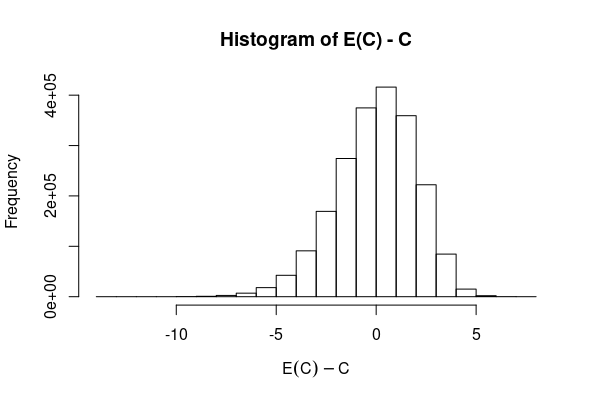
\includegraphics[scale=0.5]{images/labelling_histogram.png}
  \caption{Histogram of the difference between the expected number of vertices
    assigned each label and the actual number (for all labelled graphs)}
  \label{figure:labelling_histogram}
\end{figure}

The default value for $p$ is 33\%. The publications associated with the database
\cite{foggia2001-2, DBLP:journals/prl/SantoFSV03} say nothing about how the
labels are distributed among the $N$ values. We calculate the number of vertices
that were assigned each label for each graph (represented by $C$) and compare
those values with the numbers we would expect from a uniform distribution
(represented by $E(C)$). We plot a histogram of the difference $E(C) - C$ in
Figure \ref{figure:labelling_histogram} and observe that the difference is
normally distributed around 0.

\section{Unlabelled Graphs} \label{sec:unlabelled}
We also include a collection of benchmark instances for the subgraph isomorphism
problem\footnote{\url{http://liris.cnrs.fr/csolnon/SIP.html}} (with the
biochemical reactions dataset excluded since we are not dealing with directed
graphs). It contains only unlabelled graphs and consists of the following sets:

\begin{description}
\item[images-CVIU11] Graphs generated from segmented images. 43 pattern graphs
  and 146 target graphs, giving a total of \num{6278} instances.
\item[meshes-CVIU11] Graphs generated from meshes modelling 3D
  objects. 6 pattern graphs and 503 target graphs, giving a total of \num{3018}
  instances. Both \texttt{images-CVIU11} and \texttt{meshes-CVIU11} datasets are
  described in \cite{DBLP:journals/cviu/DamiandSHJS11}.
\item[images-PR15] Graphs generated from segmented images
  \cite{DBLP:journals/pr/SolnonDHJ15}. 24 pattern graphs and a single target
  graph, giving 24 instances.
\item[LV] Graphs with various properties (connected, biconnected, triconnected,
  bipartite, planar, etc.). 49 graphs are paired up in all possible ways, giving
  $49^2=\num{2401}$ instances.
\item[scalefree] Scale-free networks generated using a power law distribution of
  degrees (100 instances).
\item[si] Bounded valence graphs, 4D meshes, and randomly generated graphs
  (\num{1170} instances). This is the unlabelled part of the ARG database.
  \texttt{LV}, \texttt{scalefree}, and \texttt{si} datasets are described in
  \cite{DBLP:journals/ai/Solnon10, DBLP:journals/constraints/ZampelliDS10}.
\item[phase] Random graphs generated to be close to the
  satisfiable-unsatisfiable phase transition (200 instances)
  \cite{DBLP:conf/ijcai/McCreeshPT16}.
\item[largerGraphs] Larger instances of the \texttt{LV} dataset. There are 70
  graphs, giving $70^2=\num{4900}$ instances. The separation was made and used
  in \cite{DBLP:conf/aaai/HoffmannMR17, DBLP:conf/lion/KotthoffMS16,
    DBLP:conf/ijcai/McCreeshPT17}.
\end{description}

\begin{remark}
This set of instances was taken from the
repository\footnote{\url{https://github.com/jamestrimble/ijcai2017-partitioning-common-subgraph}}
for the \textsc{McSplit} paper \cite{DBLP:conf/ijcai/McCreeshPT17} and has some
minor differences from the version on Christine Solnon's website.
\end{remark}

\begin{remark}
  Since $k\downarrow$ comes from the subgraph isomorphism problem background, it
  treats the two (pattern and target) graphs differently. Therefore, when graphs
  are not divided into patterns and targets, we run the algorithms with both
  orderings ($(G_1, G_2)$ and $(G_2, G_1)$).
\end{remark}

\chapter{Generating Data} \label{chapter:generating_data}
A machine learning (ML) model requires data to learn from. We are using an R
package called \textsc{Llama} \cite{kotthoff_llama_2013, llama}, which helps to train
and evaluate ML models in order to compare algorithms and was used to create
algorithm portfolios for the travelling salesperson problem
\cite{DBLP:conf/lion/KotthoffKHT15} and the subgraph isomorphism problem
\cite{DBLP:conf/lion/KotthoffMS16}. First, we run each algorithm on all pairs of
pattern-target graphs and record the running times (described in Section
\ref{sec:runtimes}). Then, we adapt a graph feature extractor program used in
\cite{DBLP:conf/lion/KotthoffMS16} to handle the binary format of the ARG
Database \cite{foggia2001-2, DBLP:journals/prl/SantoFSV03}, run it on all
graphs, and record the features in a way described in Section
\ref{sec:features}.

\section{Running Time of Algorithms} \label{sec:runtimes}

The algorithms were compiled with gcc 6.3.0 and run on Intel Xeon E5-2697A v4
(2.60 GHz) processors with a \num{1000} s time limit. A Makefile was created to
run multiple experiments in parallel with, e.g., \texttt{make -j 64}, which
generates pairs of graph filenames for all datasets, runs the selected
algorithms with various command line arguments, redirects their output to files
that are later parsed using \texttt{sed} and regular expressions into the CSV
format. For each algorithm, we keep the full names of pattern and target graphs,
the number of vertices in the returned maximum common subgraph, running time as
reported by the algorithms themselves, and the number of explored nodes in the
search tree. Entries with running time greater than or equal to the timeout
value are considered to have timed out. The aforementioned node counts are
collected but not currently used. Afterwards, the answers of different
algorithms are checked for equality (for algorithms that did not time out).

Some limitations had to be enforced to avoid running out of memory. First, the
clique algorithm requires $O(n^2m^2)$ memory for a pair of graphs with $n$ and
$m$ vertices \cite{DBLP:conf/aaai/HoffmannMR17, DBLP:conf/cp/McCreeshNPS16}, so
its virtual memory usage was limited to 7 GB with \texttt{ulimit -v} and the
instances from Section \ref{sec:unlabelled} (which contain much larger graphs)
were restricted to $m \times n < \num{16000}$. Second, having almost $10^5$
problem instances and analysing 7 different kinds of labelling (according to
Definition \ref{def:percent_labelling}) results in too much data for the ML
algorithm. Therefore, we sample \num{30000} out of \num{81400} instances from
Section \ref{sec:labelled}. The sample is drawn once and used for training ML
models for both types of labelling. As with 50\% labelling most instances are
solved within the time limit, sampling from the whole database still leaves us
with enough relevant data.

In the rest of this section we explore and compare how the algorithms performed
on the three different subproblems under consideration, namely with unlabelled,
vertex-labelled and fully labelled graphs. We introduce
\emph{empirical cumulative distribution function (ECDF)}
plots \cite{10.2307/2334448} (also known as cumulative plots): for each unit of
time on the horizontal axis, the value on the vertical axis represents what part
of the problem instances was solved in that amount of time or less.

\subsection{Unlabelled Graphs}

\begin{figure}
  \centering
  \begin{subfigure}[t]{0.49\textwidth}
    \centering
    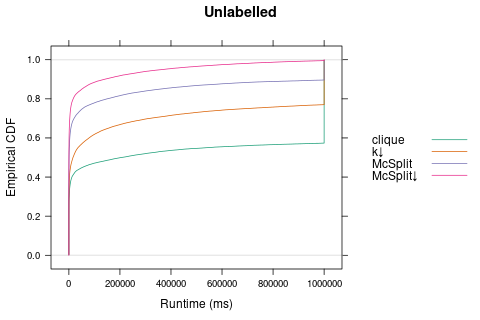
\includegraphics[width=\textwidth]{images/ecdf_mcs.png}
    \caption{Data from Section \ref{sec:labelled}, the ARG Database}
    \label{fig:ecdf_unlabelled_mcs}
  \end{subfigure}
  \begin{subfigure}[t]{0.49\textwidth}
    \centering
    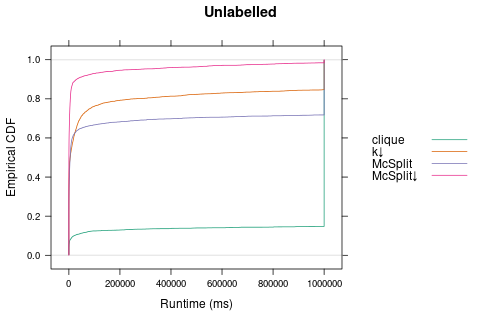
\includegraphics[width=\textwidth]{images/ecdf_sip.png}
    \caption{Data from Section \ref{sec:unlabelled}}
    \label{fig:ecdf_unlabelled_sip}
  \end{subfigure}
  \begin{subfigure}[t]{\textwidth}
    \centering
    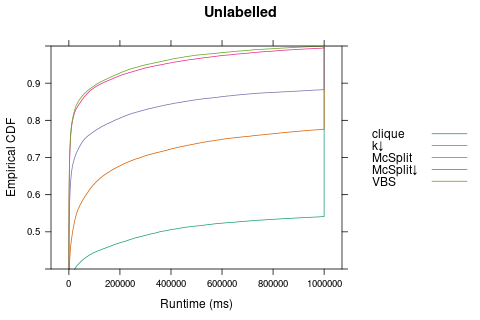
\includegraphics[width=0.49\textwidth]{images/ecdf_unlabelled.png}
    \caption{All unlabelled data}
    \label{fig:ecdf_unlabelled_both}
  \end{subfigure}
  \caption{Comparison of the runtimes of algorithms on unlabelled data}
  \label{fig:ecdf_unlabelled}
\end{figure}

We plot the ECDF plots for unlabelled graphs in both databases in Figure
\ref{fig:ecdf_unlabelled}. We can check that the orderings of the algorithms in
parts (a) and (b) of Figure \ref{fig:ecdf_unlabelled} are the same as in Figures
3a and 4 in the \textsc{McSplit} paper \cite{DBLP:conf/ijcai/McCreeshPT17}.
Namely, \textsc{McSplit} outperforms $k\downarrow$ in Figure
\ref{fig:ecdf_unlabelled_mcs}, and the opposite happens in Figure
\ref{fig:ecdf_unlabelled_sip}. In Figure \ref{fig:ecdf_unlabelled_both} we also
plot a curve for the \emph{virtual best solver (VBS)}, i.e., a perfect algorithm
portfolio that always chooses the best-performing algorithm for each problem
instance. Note that the difference between $\textsc{McSplit}\downarrow$ and VBS
is very small. Therefore, a portfolio cannot provide significant performance
benefits for this subproblem.

\begin{table}
  \centering
  \begin{tabular}{l r r r r}
    Dataset & clique & $k\downarrow$ & \textsc{McSplit} & $\textsc{McSplit}\downarrow$ \\
    \hline
    \texttt{images-CVIU11} & 0 & 32 & 79 & 1081 \\
    \texttt{images-PR15} & 0 & 0 & 0 & 24 \\
    \texttt{largerGraphs} & 0 & 14 & 30 & 167 \\
    \texttt{LV} & 90 & 30 & 489 & 439 \\
    \texttt{meshes-CVIU11} & 0 & 13 & 0 & 23 \\
    \texttt{phase} & 0 & 0 & 0 & 0 \\
    \texttt{scalefree} & 0 & 0 & 0 & 80 \\
    \texttt{si} & 0 & 10 & 102 & 1135 \\
    ARG Database & 1443 & 141 & 21965 & 27305 \\
    \hline
    Total & 1533 & 240 & 22665 & 30254
  \end{tabular}
  \caption{The number of times each algorithm was the best, for each dataset}
  \label{table:best}
\end{table}

Table \ref{table:best} shows that most of the datasets have multiple algorithms
that managed to outperform the others for some problem instances. Thus, looking
at the differences between different datasets will not be enough to predict the
best algorithm. More specifically, Table \ref{table:best} shows the numbers of
times that each algorithm's runtime was lower than or equal to the runtimes of
other algorithms. Therefore, if 2 or more lowest runtimes are equal (as can
often happen with single-digit runtimes), both algorithms are marked as winning
in the table.

Given this information, we would expect the ML algorithm to suggest using
\textsc{McSplit} and $\textsc{McSplit}\downarrow$ most of the time, occasionally
consider the clique encoding, and mostly forget about $k\downarrow$.

\subsection{Labelled Graphs} \label{sec:labelled_runtimes}

\begin{figure}
  \centering
  \begin{subfigure}[t]{0.49\textwidth}
    \centering
    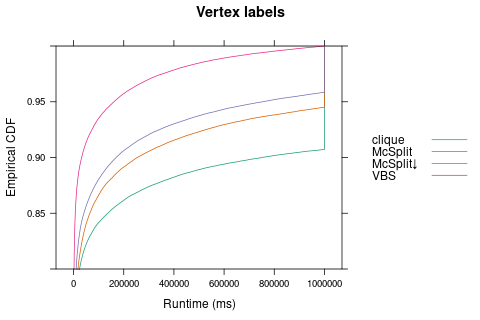
\includegraphics[width=\textwidth]{images/ecdf_vertex_labels.png}
  \end{subfigure}
  \begin{subfigure}[t]{0.49\textwidth}
    \centering
    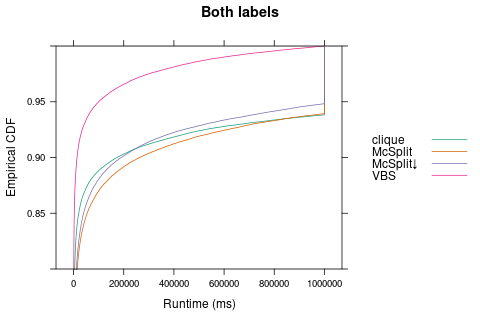
\includegraphics[width=\textwidth]{images/ecdf_both_labels.png}
  \end{subfigure}
  \caption{Cumulative plots with the vertical axis starting at 0.8}
  \label{fig:ecdfs}
\end{figure}

We deal with the two types of labelling separately, however, since the results
are fairly similar, we describe them in the same section to highlight the
differences. We plot the ECDFs in Figure \ref{fig:ecdfs}. The situation with
vertex-labelled graphs is quite straightforward: $\textsc{McSplit}\downarrow$ is
slight better than \textsc{McSplit}, which is better than the clique encoding.
Moreover, the VBS curve is significantly higher, providing plenty of room for an
ML model to outperform individual algorithms (unlike with unlabelled data). This
latter fact is true for fully labelled graphs as well, whereas
the other 3 curves provide a more interesting story. The clique algorithm is
briefly winning for shorter timeout values, then is between
$\textsc{McSplit}\downarrow$ and \textsc{McSplit} until it drops to the
3\textsuperscript{rd} place right before the final timeout at \num{1000000} ms.
This is likely because the clique encoding is better with higher labelling
percentages (we will see this shortly) and such graphs are generally easier to
solve (because there are fewer ``matchable'' combinations of vertices, each pair
of vertices is likely to have different labels).

\begin{figure}
  \centering
  \begin{subfigure}[t]{0.49\textwidth}
    \centering
    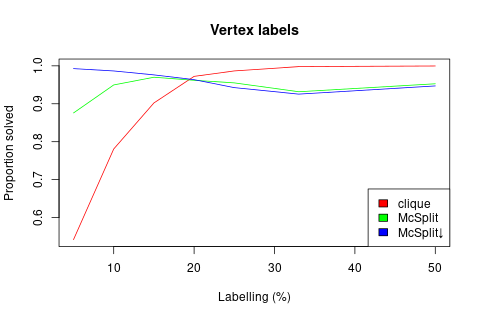
\includegraphics[width=\textwidth]{images/vertex_labels_linechart.png}
    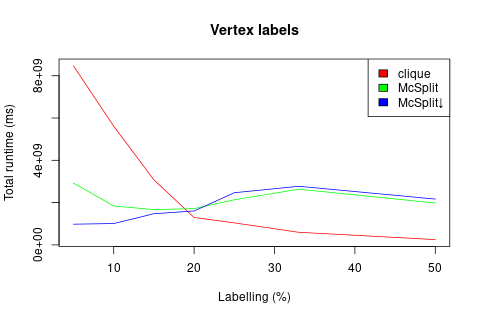
\includegraphics[width=\textwidth]{images/vertex_labels_linechart2.png}
    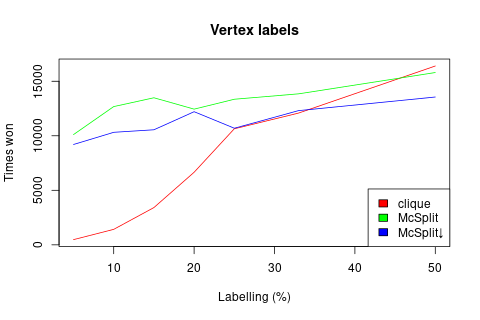
\includegraphics[width=\textwidth]{images/vertex_labels_linechart3.png}
  \end{subfigure}
  \begin{subfigure}[t]{0.49\textwidth}
    \centering
    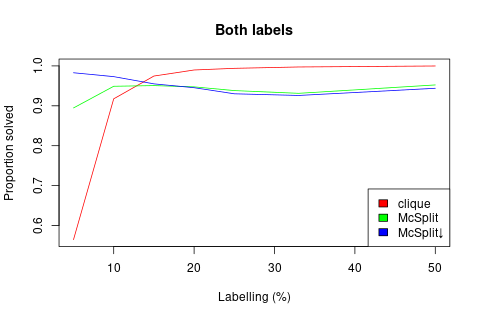
\includegraphics[width=\textwidth]{images/both_labels_linechart.png}
    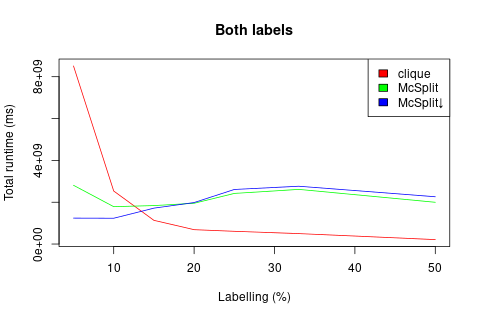
\includegraphics[width=\textwidth]{images/both_labels_linechart2.png}
    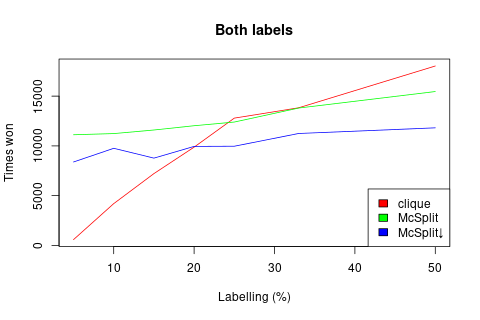
\includegraphics[width=\textwidth]{images/both_labels_linechart3.png}
  \end{subfigure}
  \caption{For both types of labelling and for the 3 algorithms we plot how the
    3 characteristics change with respect to the labelling percentage:
    proportion of instances solved within the time limit, total runtime, and
    number of times each algorithm outperformed the others}
  \label{fig:linecharts}
\end{figure}

Just like with unlabelled graphs we could split the data into different subsets
based on how (and by whom) the graphs were generated, now we can analyse how the
situation changes with different labelling percentages. In Figure
\ref{fig:linecharts} we analyse two performance measures (proportion of
instances solved and total runtime) as well as the number of times each
algorithm ``wins'', for each labelling percentage. The two performance
statistics tell exactly the same story, and it is the same for both types of
labelling. The only difference is that the clique algorithm's major drop in
performance starts at 20\% for vertex-labelled graphs and at 15\% for fully
labelled graphs. With higher labelling percentages, the clique encoding is
better than \textsc{McSplit}, which is marginally better than
$\textsc{McSplit}\downarrow$. Whereas with lower levels of labelling, two
differences emerge: \textsc{McSplit} experiences a drop in performance below
$\textsc{McSplit}\downarrow$, and the performance of the clique algorithm starts
to drop exponentially. The latter is exactly what makes the clique encoding
finish last in Figure \ref{fig:ecdfs}, even though it is in the lead for most
labelling percentages.

\begin{remark}
Note that we are only considering instances solved by at least one algorithm.
Out of the \num{30000} instances selected by our random sampling procedure, the
number of such instances ranges from 56\% with 5\% labelling to 99\% with 50\%
labelling for vertex-labelled graphs (the percentages for fully labelled graphs
are similar). Thus a (roughly) horizontal line should not be interpreted as the
algorithm performing equally well for different labelling percentages: the
performance of all algorithms improves with higher labelling percentages as the
problem becomes significantly easier. In this case we are more interested in the
differences between individual algorithms.
\end{remark}

As for the last two plots of Figure \ref{fig:linecharts}, \textsc{McSplit} is
winning more often than $\textsc{McSplit}\downarrow$. This is not surprising for
higher labelling percentages (based on the other two types of plots), but this
remains true for lower percentages as well. Perhaps this is because by
definition $\textsc{McSplit}\downarrow$ is better at handling problem instances
with a big answer. With a smaller labelling percentage, \textsc{McSplit} is more
likely to time out on those instances, contributing to
$\textsc{McSplit}\downarrow$ solving more instances than \textsc{McSplit}.
Perhaps $\textsc{McSplit}\downarrow$ is also much faster on those instances,
ensuring its lower total runtime, while consistently falling slightly behind
\textsc{McSplit} on easier instances, resulting in a lower win count. The one
significant difference between the two types of labelling is that the clique
encoding wins slightly less than $\textsc{McSplit}\downarrow$ with vertex
labels, but slightly more than \textsc{McSplit} with both vertex and edge
labels, for 25\%--33\% labelling. Finally, the main observation from this plot
is that the overall highest point is only at \num{16401} (\num{18031}) for
vertex-labelled graphs (both vertex and edge labels), just slightly above half
of the number of instances (\num{30000}) and other than the clique encoding
falling behind with $\le 15\%$ labelling, the 3 algorithms winning rates stay
similar. This makes the problem especially potent for a algorithm selection
approach.

\section{Graph Features} \label{sec:features}
The initial set of features is based on the algorithm selection paper for the
subgraph isomorphism problem \cite{DBLP:conf/lion/KotthoffMS16} and consists of
the following:

\begin{enumerate}
\item number of vertices,
\item number of edges,
\item mean degree,
\item maximum degree,
\item density,
\item mean distance between pairs of vertices,
\item maximum distance between pairs of vertices,
\item standard deviation of degrees,
\item number of loops,
\item proportion of all vertex pairs with a distance of at least 2, 3, and 4,
\item whether a graph is connected.
\end{enumerate}

\begin{definition}
For a graph $G$ with $n$ vertices and $m$ edges, the \emph{(edge) density} is
defined to be the proportion of potential edges that $G$ actually has
\cite{DBLP:books/daglib/0030488}. The standard formula used for \emph{simple}
graphs (i.e., graphs with no multiple edges or loops
\cite{DBLP:books/ws/NishizekiR04}) is
\[ \frac{m}{\binom{n}{2}} = \frac{2m}{n(n-1)}. \]
\end{definition}

Even though some of our graphs do contain multiple edges and loops, we stick to
this formula as it was used in \cite{DBLP:conf/lion/KotthoffMS16} and it does
not break the ML algorithm in any way to have the theoretical possibility of
density greater than 1.

We exclude feature extraction running time as a viable feature by itself (used
in \cite{DBLP:conf/lion/KotthoffMS16}) since it would not provide any insight
into what properties of the graph affect which algorithm is likely to achieve
the best performance. Since $k\downarrow$ and $\textsc{McSplit}\downarrow$ both
start by looking for (complete) subgraph isomorphisms, they are likely to
outperform other algorithms when both graphs are very similar and the maximum
common subgraph has (almost) as many vertices as the smaller of the two graphs.
Thus, for each feature $f$ in features 1--7 (excluding the rest to avoid
division by 0), we also add a feature for the ratio $\frac{f(G_p)}{f(G_t)}$,
where $G_p$ and $G_t$ are the pattern and target graphs, respectively.

We analyse three different types of labelling and treat them as separate
problems: no labels, vertex labels, vertex and edge labels. For the last two
types, we add a feature corresponding to $p$ defined in Definition
\ref{def:percent_labelling} and collect data for the following values of $p$:
5\%, 10\%, 15\%, 20\%, 25\%, 33\%, 50\%. The values correspond to having about
20, 10, 5, 4, 3, and 2 vertices/edges with the same label on average,
respectively.

\begin{remark}
  When working with both vertex and edge labels, we only consider using the same
  value of $p$ for both vertices and edges. This ``convention'' seems to have
  originated in a paper by the creators of the ARG Database
  \cite{DBLP:journals/jgaa/ConteFV07} and was replicated in subsequent papers on
  maximum common subgraph algorithms \cite{DBLP:conf/cp/McCreeshNPS16,
    DBLP:conf/cp/NdiayeS11}.
\end{remark}

\subsection{Distributions of Features}

\begin{figure}
  \centering
  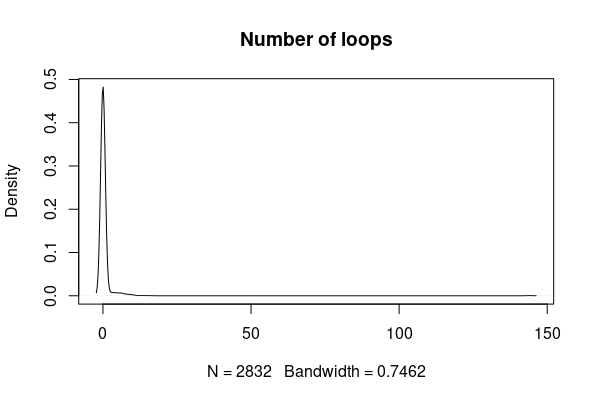
\includegraphics[scale=0.7]{images/sip_loops.png}
  \caption{Density plot of the number of loops in graphs from Section
    \ref{sec:unlabelled}}
  \label{fig:loops}
\end{figure}

\begin{figure}
  \centering
  \begin{subfigure}[t]{0.49\textwidth}
    \centering
    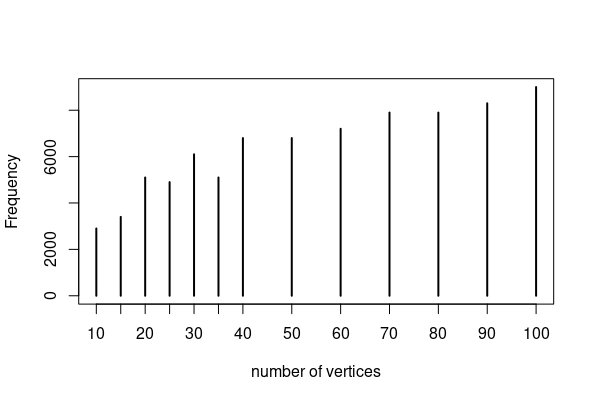
\includegraphics[width=\textwidth]{images/mcs_vertices.png}
  \end{subfigure}
  \begin{subfigure}[t]{0.49\textwidth}
    \centering
    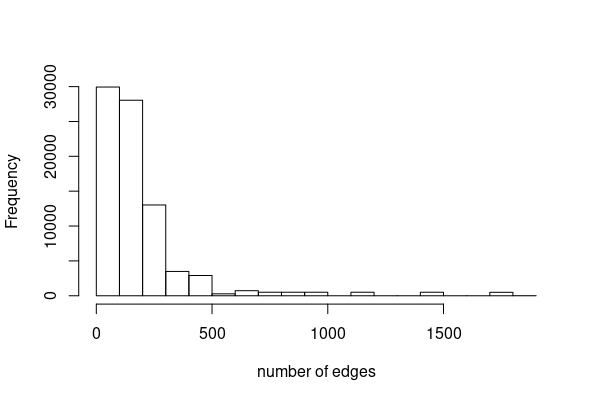
\includegraphics[width=\textwidth]{images/mcs_edges.png}
  \end{subfigure}
  \begin{subfigure}[t]{0.49\textwidth}
    \centering
    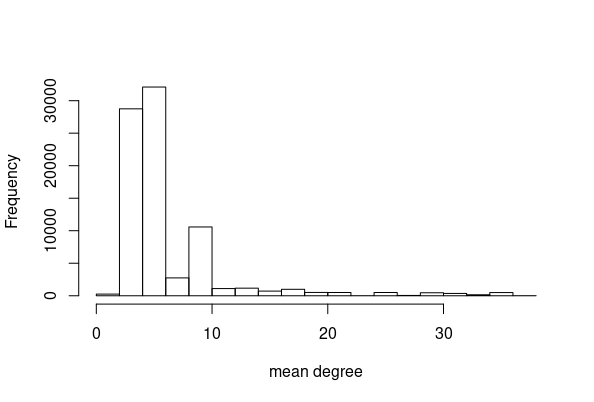
\includegraphics[width=\textwidth]{images/mcs_meandeg.png}
  \end{subfigure}
  \begin{subfigure}[t]{0.49\textwidth}
    \centering
    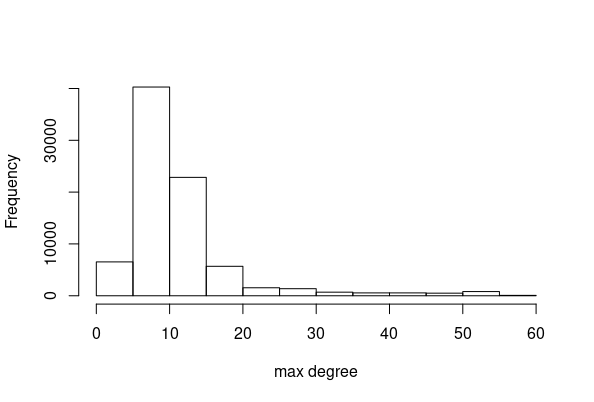
\includegraphics[width=\textwidth]{images/mcs_maxdeg.png}
  \end{subfigure}
  \begin{subfigure}[t]{0.49\textwidth}
    \centering
    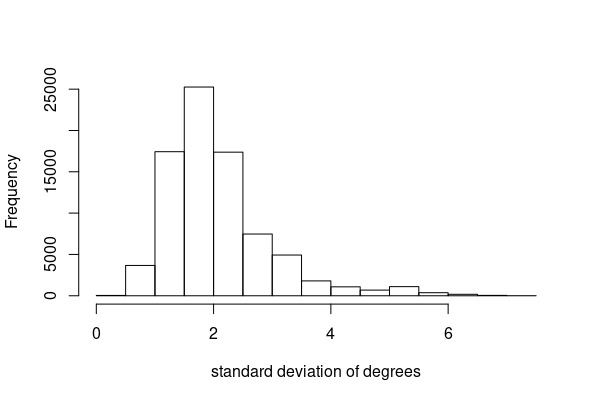
\includegraphics[width=\textwidth]{images/mcs_stddeg.png}
  \end{subfigure}
  \begin{subfigure}[t]{0.49\textwidth}
    \centering
    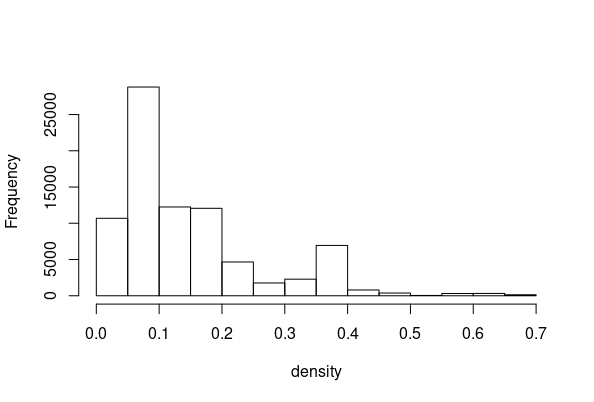
\includegraphics[width=\textwidth]{images/mcs_density.png}
  \end{subfigure}
  \begin{subfigure}[t]{0.49\textwidth}
    \centering
    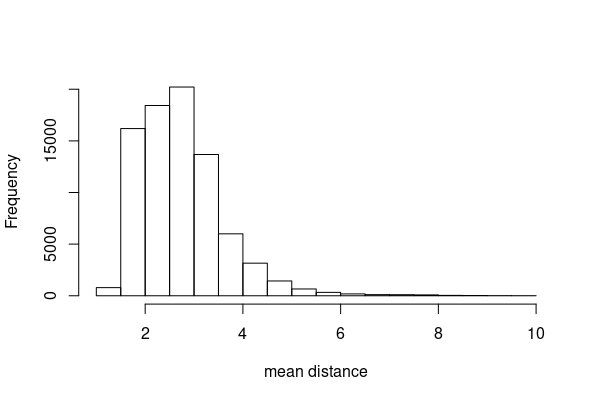
\includegraphics[width=\textwidth]{images/mcs_meandist.png}
  \end{subfigure}
  \begin{subfigure}[t]{0.49\textwidth}
    \centering
    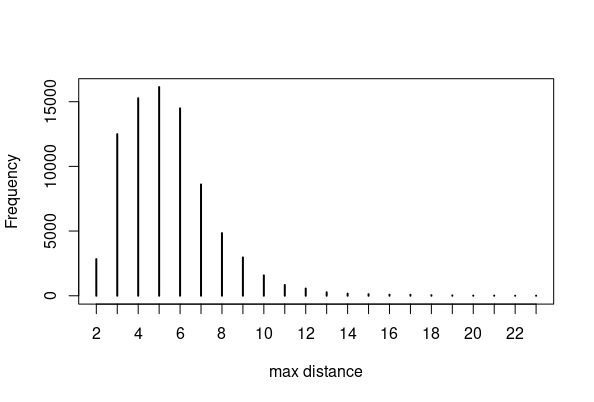
\includegraphics[width=\textwidth]{images/mcs_maxdist.png}
  \end{subfigure}
  \caption{Plots of how various features are distributed for graphs from Section
  \ref{sec:labelled}}
  \label{fig:mcs_features1}
\end{figure}

\begin{figure}
  \centering
  \begin{subfigure}[t]{0.49\textwidth}
    \centering
    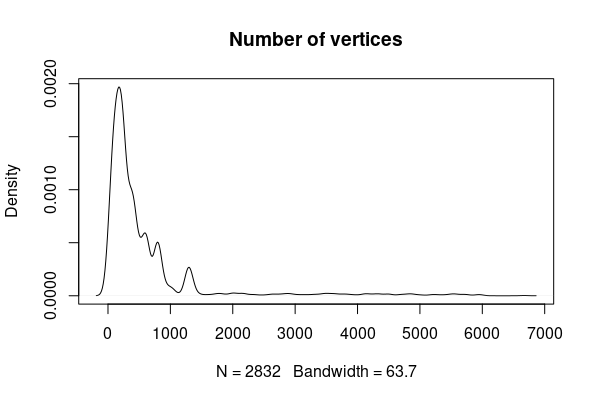
\includegraphics[width=\textwidth]{images/sip_vertices.png}
  \end{subfigure}
  \begin{subfigure}[t]{0.49\textwidth}
    \centering
    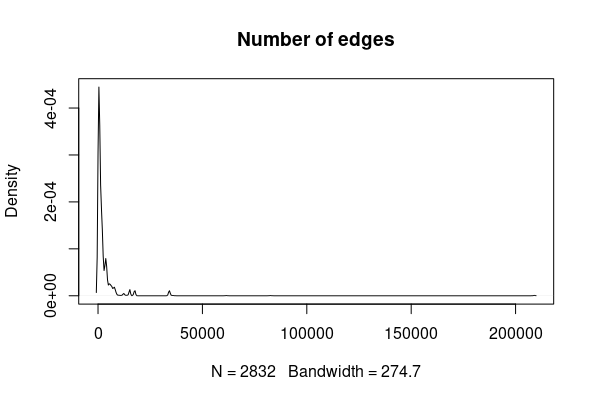
\includegraphics[width=\textwidth]{images/sip_edges.png}
  \end{subfigure}
  \begin{subfigure}[t]{0.49\textwidth}
    \centering
    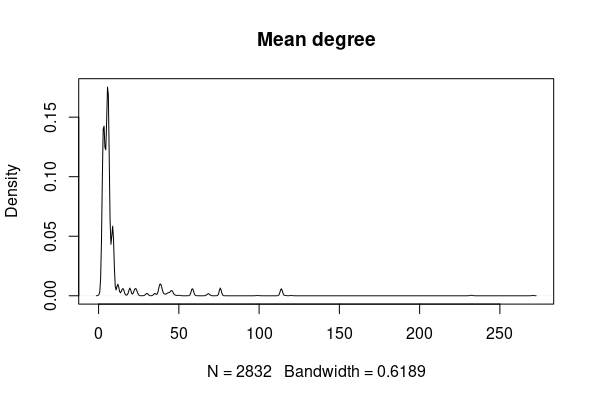
\includegraphics[width=\textwidth]{images/sip_meandeg.png}
  \end{subfigure}
  \begin{subfigure}[t]{0.49\textwidth}
    \centering
    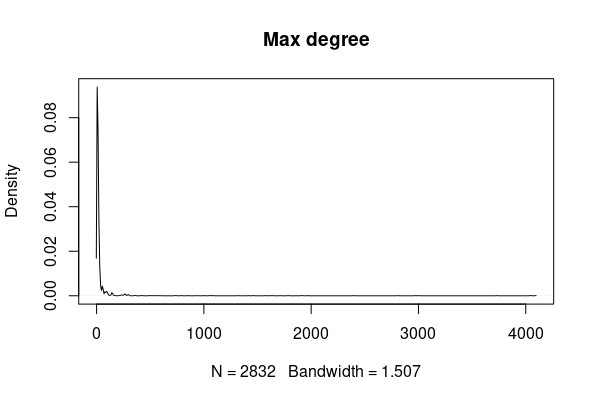
\includegraphics[width=\textwidth]{images/sip_maxdeg.png}
  \end{subfigure}
  \begin{subfigure}[t]{0.49\textwidth}
    \centering
    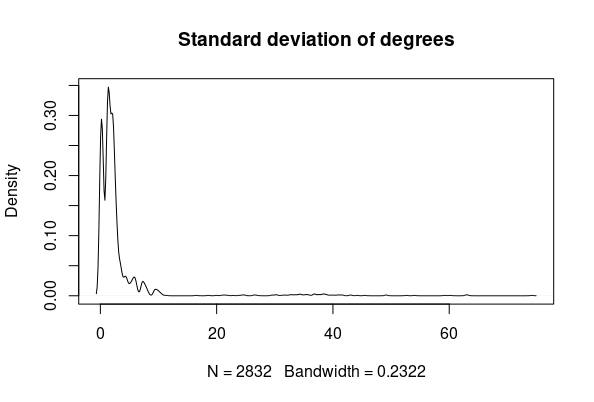
\includegraphics[width=\textwidth]{images/sip_stddeg.png}
  \end{subfigure}
  \begin{subfigure}[t]{0.49\textwidth}
    \centering
    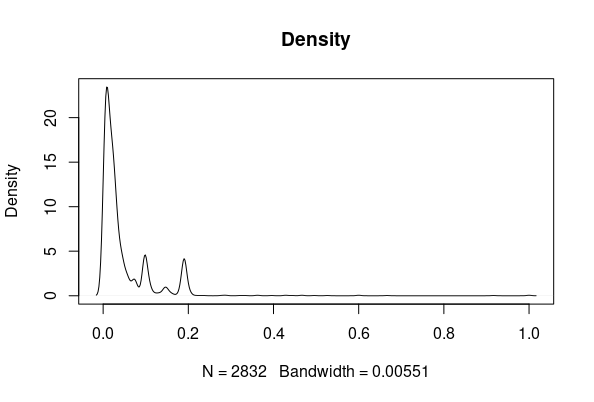
\includegraphics[width=\textwidth]{images/sip_density.png}
  \end{subfigure}
  \begin{subfigure}[t]{0.49\textwidth}
    \centering
    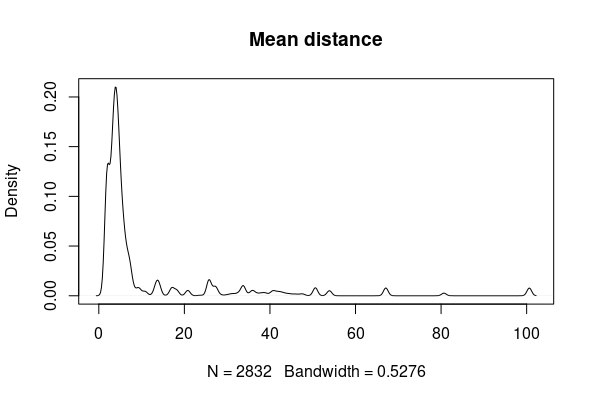
\includegraphics[width=\textwidth]{images/sip_meandist.png}
  \end{subfigure}
  \begin{subfigure}[t]{0.49\textwidth}
    \centering
    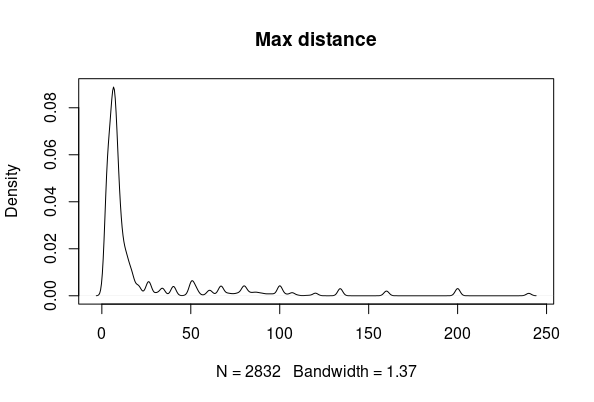
\includegraphics[width=\textwidth]{images/sip_maxdist.png}
  \end{subfigure}
  \caption{Plots of how various features are distributed for graphs from Section
  \ref{sec:unlabelled}}
  \label{fig:sip_features1}
\end{figure}

\begin{figure}
  \centering
  \begin{subfigure}[t]{0.49\textwidth}
    \centering
    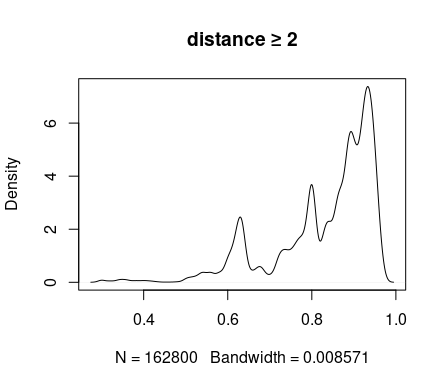
\includegraphics[width=\textwidth]{images/mcs_prop2.png}
  \end{subfigure}
  \begin{subfigure}[t]{0.49\textwidth}
    \centering
    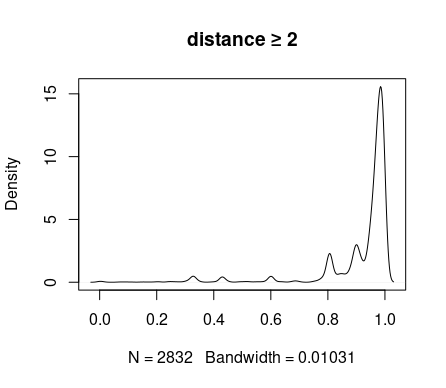
\includegraphics[width=\textwidth]{images/sip_prop2.png}
  \end{subfigure}
  \begin{subfigure}[t]{0.49\textwidth}
    \centering
    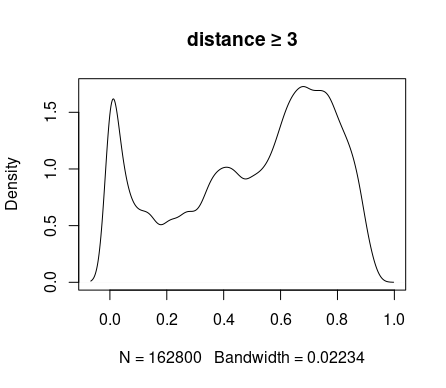
\includegraphics[width=\textwidth]{images/mcs_prop3.png}
  \end{subfigure}
  \begin{subfigure}[t]{0.49\textwidth}
    \centering
    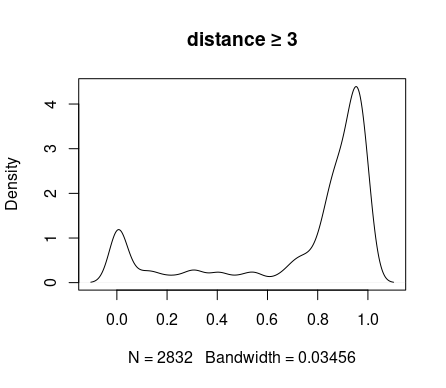
\includegraphics[width=\textwidth]{images/sip_prop3.png}
  \end{subfigure}
  \begin{subfigure}[t]{0.49\textwidth}
    \centering
    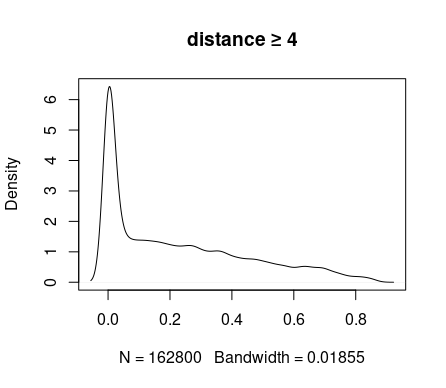
\includegraphics[width=\textwidth]{images/mcs_prop4.png}
  \end{subfigure}
  \begin{subfigure}[t]{0.49\textwidth}
    \centering
    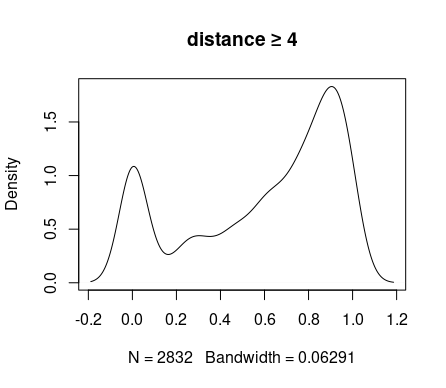
\includegraphics[width=\textwidth]{images/sip_prop4.png}
  \end{subfigure}
  \caption{Comparison of typical distances between pairs of vertices between the
  two graph databases with graphs from Section \ref{sec:labelled} on the left
  and graphs from Section \ref{sec:unlabelled} on the right}
  \label{fig:proportions}
\end{figure}

\begin{figure}
  \centering
  \begin{subfigure}[t]{0.49\textwidth}
    \centering
    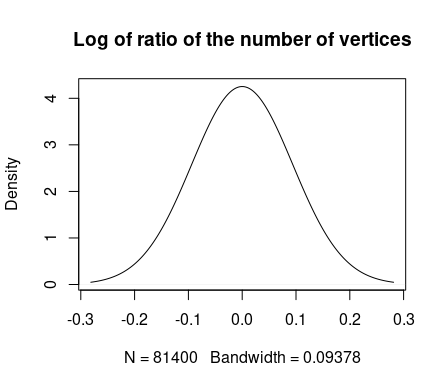
\includegraphics[width=\textwidth]{images/mcs_ratio_vertices.png}
  \end{subfigure}
  \begin{subfigure}[t]{0.49\textwidth}
    \centering
    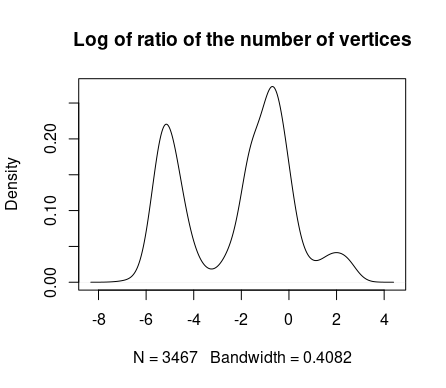
\includegraphics[width=\textwidth]{images/sip_ratio_vertices.png}
  \end{subfigure}
  \caption{The density plots of log-transformed ratio of the number of vertices
    between pattern and target graphs for both databases with graphs from
    Section \ref{sec:labelled} on the left and graphs from Section
    \ref{sec:unlabelled} on the right}
  \label{fig:ratio_vertices}
\end{figure}

\begin{figure}
  \centering
  \begin{subfigure}[t]{0.49\textwidth}
    \centering
    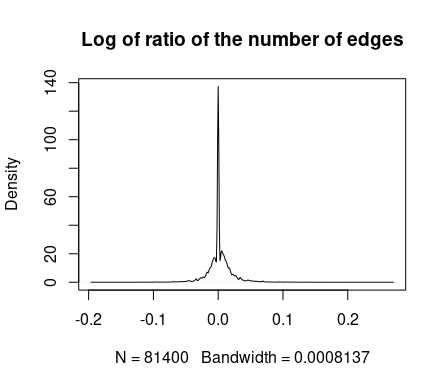
\includegraphics[width=\textwidth]{images/mcs_ratio_edges.png}
  \end{subfigure}
  \begin{subfigure}[t]{0.49\textwidth}
    \centering
    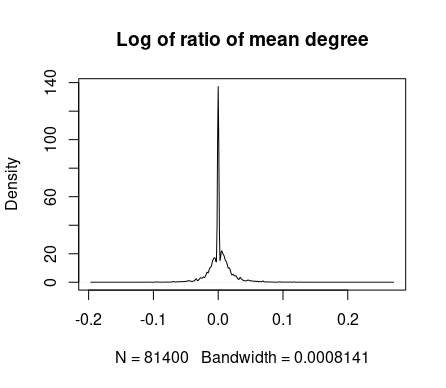
\includegraphics[width=\textwidth]{images/mcs_ratio_meandeg.png}
  \end{subfigure}
  \begin{subfigure}[t]{0.49\textwidth}
    \centering
    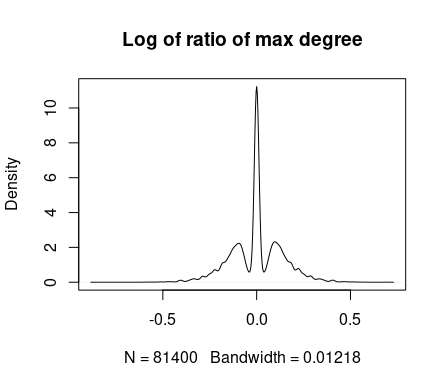
\includegraphics[width=\textwidth]{images/mcs_ratio_maxdeg.png}
  \end{subfigure}
  \begin{subfigure}[t]{0.49\textwidth}
    \centering
    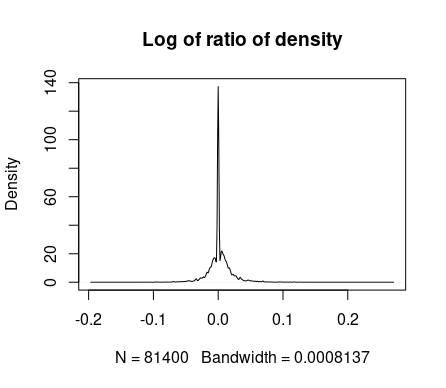
\includegraphics[width=\textwidth]{images/mcs_ratio_density.png}
  \end{subfigure}
  \begin{subfigure}[t]{0.49\textwidth}
    \centering
    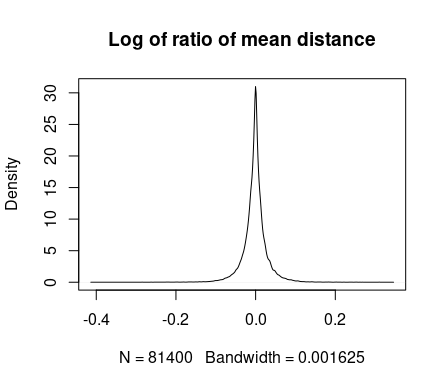
\includegraphics[width=\textwidth]{images/mcs_ratio_meandist.png}
  \end{subfigure}
  \begin{subfigure}[t]{0.49\textwidth}
    \centering
    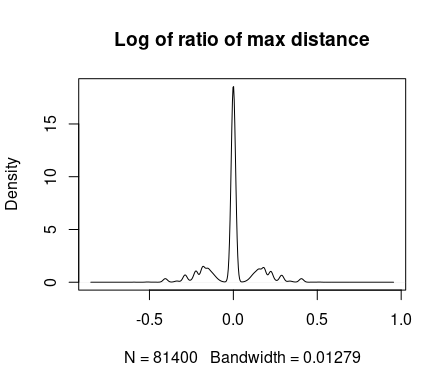
\includegraphics[width=\textwidth]{images/mcs_ratio_maxdist.png}
  \end{subfigure}
  \caption{The other density plots of the log-transformed ratio features for
    graphs from Section \ref{sec:labelled}}
  \label{fig:mcs_ratio}
\end{figure}

\begin{figure}
  \centering
  \begin{subfigure}[t]{0.49\textwidth}
    \centering
    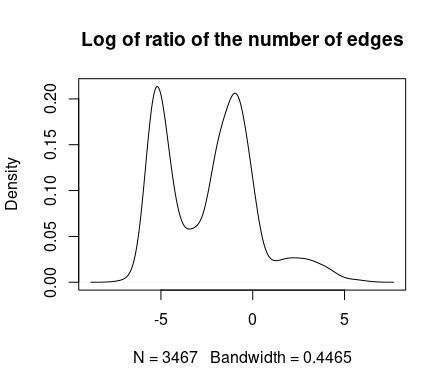
\includegraphics[width=\textwidth]{images/sip_ratio_edges.png}
  \end{subfigure}
  \begin{subfigure}[t]{0.49\textwidth}
    \centering
    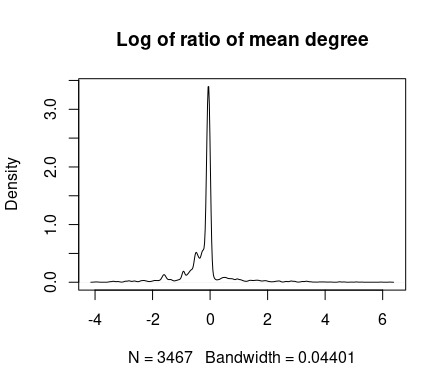
\includegraphics[width=\textwidth]{images/sip_ratio_meandeg.png}
  \end{subfigure}
  \begin{subfigure}[t]{0.49\textwidth}
    \centering
    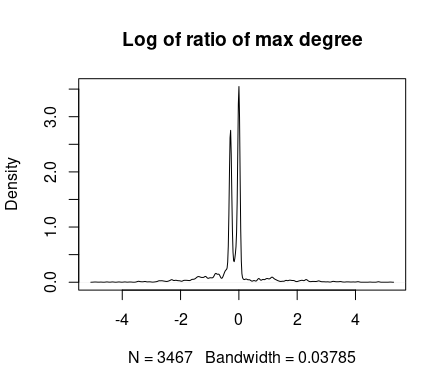
\includegraphics[width=\textwidth]{images/sip_ratio_maxdeg.png}
  \end{subfigure}
  \begin{subfigure}[t]{0.49\textwidth}
    \centering
    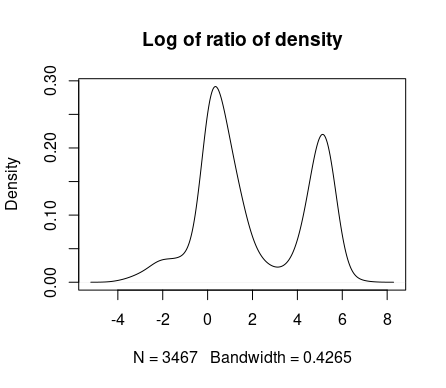
\includegraphics[width=\textwidth]{images/sip_ratio_density.png}
  \end{subfigure}
  \begin{subfigure}[t]{0.49\textwidth}
    \centering
    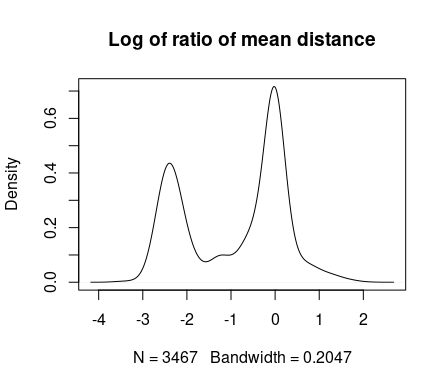
\includegraphics[width=\textwidth]{images/sip_ratio_meandist.png}
  \end{subfigure}
  \begin{subfigure}[t]{0.49\textwidth}
    \centering
    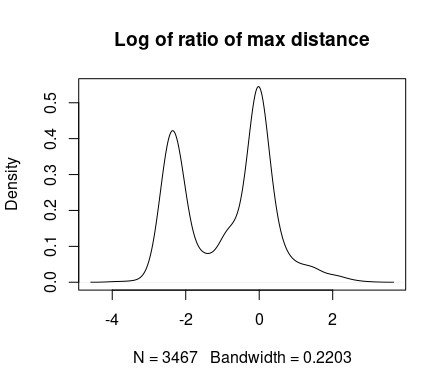
\includegraphics[width=\textwidth]{images/sip_ratio_maxdist.png}
  \end{subfigure}
  \caption{The other density plots of the log-transformed ratio features for
    graphs from Section \ref{sec:unlabelled}}
  \label{fig:sip_ratio}
\end{figure}

In this section we plot and discuss how the selected features are distributed in
both databases. As the graphs from Section \ref{sec:unlabelled} contain some
very hard instances, we only consider graphs that are part of a pair of graphs
solved by at least one algorithm. In order to visualise highly skewed data, we
sometimes use density plots. Furthermore, we take $\log$ transformations of
ratio features.

Firstly, one feature is not plotted as by definition it has only two possible
values. 99.81\% of graphs from Section \ref{sec:labelled} are connected,
compared to 93.19\% of graphs from Section \ref{sec:unlabelled}. As both numbers
are quite high, they may not be ideal for establishing if connectedness is a
significant factor in determining which algorithm performs the best, but might
be representative of real data in application domains such as chemistry
\cite{WCMS:WCMS5}. Similarly, the number of loops for graphs from Section
\ref{sec:labelled} is not plotted as it varies between two values: 0.98\% of the
graphs have a single loops, while the remaining majority of graphs have no
loops. On the other hand, as shown in Figure \ref{fig:loops}, some (although not
many) graphs from Section \ref{sec:unlabelled} have significantly more loops.

Most of the features of graphs from Section \ref{sec:labelled} are displayed in
Figure \ref{fig:mcs_features1}. Other than the number of vertices, which is
manually controlled by the creators of the database, all other distributions are
centred around lower values, with some outliers on the high end. More
importantly, we have some graphs that are quite dense and some graphs with
higher mean distance values.

The same plots for graphs from Section \ref{sec:unlabelled} in Figure
\ref{fig:sip_features1} show a similar story, albeit for clearer reasons. Since
we filter out graphs that none of the algorithms were able to handle, our sample
consists of all the easy instances and some harder instances that were
solved by one or two algorithms. Harder instances typically have more vertices,
which means they are also capable of higher values for many other features,
hence all of the density plots are right skewed.

Figure \ref{fig:proportions} shows density plots of proportions of pairs of
vertices with distance at least $k$ for $k = 2, 3, 4$. For both databases, as
$k$ increases, the distributions shift to the left as expected. However, there
is one important difference: even with $k = 4$ the plot for graphs from Section
\ref{sec:unlabelled} has its highest peak around 0.9, which means that adding
features for $k \ge 5$ could be valuable.

Finally, the density plots of $\log$-transformed ratio features are in Figures
\ref{fig:ratio_vertices}, \ref{fig:mcs_ratio}, and \ref{fig:sip_ratio}. Almost
all of these plots for graphs from Section \ref{sec:unlabelled} (with the
exception of the ratio of mean degree) are clearly bimodal with one of the two
modes centred around 0. Hence we can infer the existence of two subpopulations:
one where pattern and target graphs have very similar properties (the majority
for most features) and one where pattern and target graphs are very different.
As for the graphs from Section \ref{sec:labelled}, the plot of the ratio of the
number of vertices in Figure \ref{fig:ratio_vertices} is perfectly symmetrical
and centred around 0, since the number of vertices is a controlled variable for
this database. All of the remaining plots for ratio features have most of the
data very close to 0. Thus, the differences between pattern and target graphs
are very small. Furthermore, all distributions are symmetrical---the
pattern graph is just as likely to be larger/denser/etc. as the opposite.

\chapter{Machine Learning Models \& Their Evaluation}

After running the algorithms  with different types and percentages of labelling
and recording their running times, an ML algorithm can be trained to predict which
algorithm should be chosen for each pair of graphs. For each pair of graphs,
\textsc{Llama} \cite{llama} can take:

\begin{itemize}
\item A list of features. With separate features for pattern and target graphs
  as well as ratio features and the labelling percentage, we have 34 features in
  total.
\item A list of performance measures for all algorithms, i.e., the values that
  we are trying to optimise. In this case (as in most cases), this corresponds
  to running time. The values are capped at the timeout value (\num{1000000} ms).
  Furthermore, instances that were not run on the clique algorithm are also set
  to the timeout value. Finally, we filter out instances where all of the
  algorithms timed out.
\item A list of Boolean values, denoting whether each algorithm successfully
  finished or not. Timeouts, the clique algorithm running out of memory, and
  instances that were not run with the clique algorithm because of their size
  are all marked as false.
\item A data frame, measuring the running time taken to compute each feature for
  each problem instance, a single number for the approximate time taken to
  compute all features for any instance, or a list with one or more costs per
  problem instance. We use the last option with a single cost per instance. This
  parameter is used to ensure a fair comparison when comparing the portfolio
  against other algorithms: the runtime of the portfolio is defined as the
  runtime of its chosen algorithm together with feature extraction time.
  While costs for graphs from Section \ref{sec:unlabelled} reached up to 65 s,
  the maximum cost for graphs from Section \ref{sec:labelled} is only 6 ms.
\end{itemize}

After constructing the required data frames as described above, the data needs to
be split into training and test sets. We use a technique called 10-fold
\emph{cross-validation}, which splits the data into 10 parts \cite{citeulike:1304145}.
9/10\textsuperscript{ths} of the data is used to train the ML algorithm, while
the remaining 1/10\textsuperscript{th} is used to evaluate how good the trained
model is. This process of training and evaluation is repeated 10 times, letting
each of the 10 parts be used for evaluation exactly once. The goodness-of-fit
criteria are then averaged out between the 10 runs.

The 10 folds could, of course, be chosen completely randomly. However, research
suggests that stratified cross-validation typically outperforms
random-sampling-based cross-validation and results in a better model
\cite{DBLP:conf/ijcai/Kohavi95}. Suppose we have a dataset of $N$ elements.
\emph{Stratified sampling} partitions it into a number of subpopulations $s_1,
\dots, s_k$ with $n_1, \dots, n_k$ elements, respectively (typically based on
the value of some feature or collection of features). It then draws from each
subpopulation independently, ensuring that approximately $n_i/N$ of the sample
comes from subpopulation $s_i$ for $i = 1, \dots, k$ \cite{lohr2009sampling}. In
this case the data is partitioned into four groups based on which algorithm
performed best.

The cross-validation folds are then used to generate predictions on all data,
where each prediction is made by a model that did not have that observation in
its training data set. The predictions are then used to compare the ML model with
individual algorithms and the VBS using ECDF plots and numeric statistics.
\textsc{Llama} \cite{kotthoff_llama_2013, llama} supports algorithm portfolios
based on three different types of ML algorithms:

\begin{description}
  \item[Classification] The ML algorithm predicts which algorithm is likely to
    perform best on each problem instance.
  \item[Regression] Each algorithm's data is used to train a separate ML model,
    predicting the algorithm's performance. The winning algorithm can then be
    chosen based on those predictions.
  \item[Clustering] All instances of the training data are clustered and the
    best algorithm is determined for each cluster. New problem instances can
    then be assigned to the nearest cluster.
\end{description}

We are using a classification algorithm called random forests
\cite{DBLP:journals/ml/Breiman01}, implemented in R \cite{randomforest}. We
chose this algorithm as it is recommended in the \textsc{Llama} manual
\cite{kotthoff_llama_2013} and successfully used in a similar study
\cite{DBLP:conf/lion/KotthoffMS16}. We use the default number of trees (500),
and our trees have about \num{6000}, \num{20000}, and \num{21000} vertices on
average for unlabelled, vertex-labelled, and fully labelled graphs,
respectively.

In order to discuss and analyse the ML algorithm in more detail, we introduce
some new terminology. Each problem instance with features and running times in
the training dataset is called an \emph{observation}. The \emph{class} of an
observation is the algorithm with lowest running time for that problem instance.
Previously discussed features of graphs are sometimes referred to as
\emph{(independent) variables}. The \emph{(problem) instance space} is the
Cartesian product of the domains of features \cite{DBLP:series/smpai/RokachM14},
where a \emph{domain} of $X$ (denoted $\dom X$) is a set of all possible values
that $X$ can take.

A \emph{(classification) decision tree} is ``a classifier expressed as a
recursive partition of the instance space'' \cite{DBLP:series/smpai/RokachM14}.
Typically, it can be represented as a rooted binary tree, where each internal
node \emph{splits} the instance space into two regions based on the value of one
of the features. For example, for some feature $X$ and a particular value $x \in
\dom{X}$, the left child might be assigned all observations with $X < x$, while
the right child would get observations with $X \ge x$. For each leaf node, we
can count how many of its observations belong to each class and assign the most
common class to that node.

\begin{remark}
  Other possibilities include a node having more than two children and a split
  being made in a more complicated way. Although trees with such properties fit
  the definition of a decision tree, standard machine learning algorithms tend
  to be more restrictive \cite{James:2014:ISL:2517747,
    DBLP:series/smpai/RokachM14}.
\end{remark}

When a decision tree is used to make a classification prediction, a data point
travels from node to node (starting at the root node) according to the splitting
rules. When it reaches a leaf node, the class assigned to that node is outputted
as the tree's prediction.

A \emph{random forest} builds a collection of decision trees
\cite{James:2014:ISL:2517747}. Given $p$ variables, each time a split is
considered, the variable to split on is chosen from $\sqrt{p}$ rather than all
$p$ variables. Therefore, the strongest predictors are sometimes not even
considered, ensuring a level of diversity among trees. An individual tree's
prediction is called a \emph{vote}. A classifying random forest predicts by
collecting the votes from all its trees and predicting the class with the
highest number of votes.

As we saw in Section \ref{sec:features}, some of the feature data is highly
skewed. Thus we should formally address the question of using transformations
(such as $\log$ used for some of the plots or $x \mapsto 1/x$, giving
the labelling percentage a different interpretation) before feeding the
data into the ML algorithm. While it is a commonly held belief that
predictor transformations are unnecessary for decision tree-based learning
algorithms \cite{DBLP:journals/classification/Friedman06,
  DBLP:books/lib/HastieTF09, cart}, they can affect the predictions of
previously unseen data \cite{DBLP:journals/corr/GaliliM16}. To see this,
consider a split between some values $x_1, x_2 > 0$ at $b =
\frac{x_1+x_2}{2}$ (which is the type of split used by the
\texttt{randomForest} package we are using
\cite{DBLP:journals/corr/GaliliM16}) and consider the same situation after
applying the transformation $x \mapsto x^2$. The new boundary is $b' =
\frac{x_1^2+x_2^2}{2}$ and it is easy to find $x > b$ such that $x^2 < b'$.
Then, if this is the final split and $x_1$ and $x_2$ have different predictions,
$x$ will have different predictions with and without the transformation. In
this project we do not use transformations as having over \num{100000} data
points and 500 trees reduces this effect and good algorithm portfolios are
created without even mentioning transformations
\cite{DBLP:conf/lion/KotthoffKHT15, DBLP:conf/lion/KotthoffMS16}. However, we
would encourage future researchers to consider $\log$-transforming highly skewed
features, especially if using an algorithm more sensitive to the distribution of
data.

Lastly, we use the \texttt{parallelMap} package to train the model using
multiple threads and the R code was heavily optimised to remove temporary
variables as soon as they are no longer needed in order to reduce memory
consumption. 

\section{Unlabelled Graphs}

\subsection{Error Rates} \label{sec:unlabelled_error_rates}

\begin{figure}
  \centering
  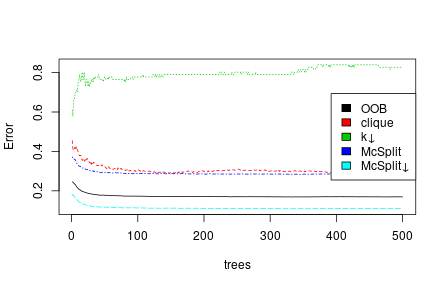
\includegraphics[scale=0.5]{images/unlabelled_forest_errors.png}
  \caption{Convergence plot of various error measures as the number of trees in
    a random forest increases. The plot shows the OOB error and $1 -
    \text{recall}$ for each algorithm.}
  \label{fig:unlabelled_forest_errors}
\end{figure}

Random forests support a convenient way to estimate the test error without
cross-validation or any other kind of data splitting. Each tree in a random
forest uses around 2/3 of the data \cite{James:2014:ISL:2517747}. The remaining
1/3 is referred to as \emph{out-of-bag (OOB)} observations . For each
observation in the data, we can predict the answer (the vote on which algorithm
is expected to win) using all trees that have the observation as OOB. The
majority vote is then declared to be the answer. The \emph{OOB error} is
the relative frequency of incorrect predictions \cite{James:2014:ISL:2517747}.
As each prediction was made using trees that had not seen that particular
observation before, OOB error is a valid estimate of test error. The black line
in Figure \ref{fig:unlabelled_forest_errors} shows how the error converges to
about 17\% as we number of trees reaches 500.

The other lines in the figure, one for each algorithm, are defined as $1 -
\text{recall}$, where, for an algorithm $A$, \emph{recall}
\cite{citeulike:12882259} is
\[ \frac{\text{the number of instances that were correctly predicted as
      $A$}}{\text{the number of instances where $A$ is the correct
      prediction}}. \]

The error rates for $\textsc{McSplit}\downarrow$, \textsc{McSplit}, the clique
encoding, and $k\downarrow$ converge to 11\%, 29\%, 30\%, and 80\%,
respectively. Unlike the errors of other classes, the error of $k\downarrow$ has
an upward trend and converges to a very high value. Perhaps the model eventually
learns not to predict $k\downarrow$ and the data points with $k\downarrow$
winning are treated as randomness in the data more so than a statistically
significant trend.

\subsection{Variable Importance}

Next we are going to explore how important each feature is in making
predictions, but for that we need to introduce some new definitions. Consider a
single tree $T$ in a random forest. The root of $T$ can be reached by any
observation, regardless of the values of its features. After passing some node
$n$, some feature is restricted, i.e., it is imposed an upper or lower limit on
the kind of values it can have for it to move towards a particular child of $n$
\cite{James:2014:ISL:2517747}. We will refer to a part of feature space that an
observation can be in while at some node $n$ as a \emph{region}.

\begin{definition}
  Suppose we have $K$ classes. Consider some region $m$. The \emph{Gini index}
  is then defined as
  \[ G = \sum_{k=1}^K \hat{p}_{mk}(1-\hat{p}_{mk}), \]
  where $\hat{p}_{mk}$ represents the proportion of observations in region $m$
  that are from class $k$ (i.e., have algorithm $k$ as the best algorithm)
  \cite{James:2014:ISL:2517747}.
\end{definition}

As we move down a tree, we want the region to be restricted to a single class.
Then the observations from the training data satisfying the conditions imposed
by the parent nodes would be classified with perfect accuracy. The Gini index is
at its lowest when all proportions $\hat{p}_{mk}$ are close to either 0 or
1\footnote{Note that $G=0$ when any single $\hat{p}_{mk}=0$, regardless of the
  values of other proportions. Therefore, $G=0$ does not automatically make a
  tree into a good classifier.}, meaning that almost all observations in the
region belong to a single class. Hence the Gini index is often used to evaluate
the quality of a split.

\begin{figure}
  \centering
  \begin{subfigure}[t]{0.45\textwidth}
    \centering
    \includegraphics[width=\textwidth]{images/unlabelled_variable_importance.png}
    \caption{Dot chart of variable importance calculated based on the Gini index
      and sorted from most important to least important}
    \label{fig:unlabelled_variable_importance}
  \end{subfigure}
  \hfill
  \begin{subfigure}[t]{0.45\textwidth}
    \centering
    \includegraphics[width=\textwidth]{images/unlabelled_var_used.png}
    \caption{How often was each variable used to make splitting decisions?}
    \label{fig:unlabelled_var_used}
  \end{subfigure}
\end{figure}

The variable importance measure of feature $f$ in Figure
\ref{fig:unlabelled_variable_importance} is calculated as the amount by which
the Gini index decreases after passing nodes that use feature $f$, averaged over
all trees in the random forest \cite{James:2014:ISL:2517747}. Looking at the
figure more closely, the standard deviations of degrees of both target and
pattern graphs are by far the most important predictors. Unsurprisingly, the
worst predictors are the features with very low variance: number of loops and
connectedness of both graphs. Perhaps more surprisingly, the ratio features are
not as successful as one might have hoped: the ratio of the numbers of vertices
is at the bottom 5\textsuperscript{th} place and the best ratio feature, the
mean distance ratio, is only 10\textsuperscript{th}. Last thing to note is that
features of the pattern graph are always behind the same features of the target
graph and usually not far behind. Perhaps this is due to some datasets having
less pattern graphs, or pattern graphs having fewer vertices. The variable usage
plot in Figure \ref{fig:unlabelled_var_used} tells a similar story: the orders
are not identical, but there are no big outliers.

\subsection{Margins}

\begin{definition}
  Let $c_1, \dots, c_n$ be $n$ classes and let $p$ be a data point that belongs
  to class $c_p$. Let $v_1, \dots, v_n$ denote the number of votes for each
  class when given $p$ as input. The \emph{margin} of $p$ is
  \[ \frac{v_p}{\sum_{i=1}^n v_i} - \max_{i \ne p} \frac{v_i}{\sum_{j=1}^n v_j}, \]
  which is a number in $[-1, 1]$ \cite{forest}.
\end{definition}

\begin{figure}
  \centering
  \begin{subfigure}[t]{0.49\textwidth}
    \centering
    \includegraphics[width=\textwidth]{images/unlabelled_margin.png}
    \caption{Sorted}
    \label{fig:unlabelled_margins1}
  \end{subfigure}
  \begin{subfigure}[t]{0.49\textwidth}
    \centering
    \includegraphics[width=\textwidth]{images/unlabelled_margin2.png}
    \caption{Unsorted}
    \label{fig:unlabelled_margins2}
  \end{subfigure}
  \caption{Margins of the data points}
  \label{fig:unlabelled_margins}
\end{figure}

\begin{figure}
  \centering
  \begin{subfigure}[t]{0.49\textwidth}
    \centering
    \includegraphics[width=\textwidth]{images/clique_hist.png}
  \end{subfigure}
  \begin{subfigure}[t]{0.49\textwidth}
    \centering
    \includegraphics[width=\textwidth]{images/kdown_hist.png}
  \end{subfigure}
  \begin{subfigure}[t]{0.49\textwidth}
    \centering
    \includegraphics[width=\textwidth]{images/mcsplit_hist.png}
  \end{subfigure}
  \begin{subfigure}[t]{0.49\textwidth}
    \centering
    \includegraphics[width=\textwidth]{images/mcsplitdown_hist.png}
  \end{subfigure}
  \caption{Histograms of margins for each winning algorithm}
  \label{fig:unlabelled_margin_hist}
\end{figure}

A value above 0 means that the forest as a whole predicted correctly. A margin
of 1 would mean that all trees voted correctly. In Figure
\ref{fig:unlabelled_margins} we plot the margins in the following way: for each
problem instance, the colour signifies the winning algorithm and the height
shows its margin. Figure \ref{fig:unlabelled_margins1} shows the points sorted
by the margin, while in Figure \ref{fig:unlabelled_margins2} they are left in
the original order of the data (which mostly corresponds to the order of files
in the databases, but with some variation since experiments are started in order
but end at different times). We can recognise the same error rates as in Figure
\ref{fig:unlabelled_forest_errors} as well as areas where \textsc{McSplit} and
$\textsc{McSplit}\downarrow$ dominate. We also plot the histograms of how the
margins are distributed for each algorithm in Figure
\ref{fig:unlabelled_margin_hist}. We note that:

\begin{itemize}
\item Instances best handled with the clique encoding are usually recognised, but
  with significant uncertainty.
\item We are usually wrong about $k\downarrow$ (probably because it is a
  winning algorithm in only 0.44\% of all cases).
\item When faced with an instance that is best handled with
  $\textsc{McSplit}\downarrow$, the vast majority of trees vote correctly.
\item \textsc{McSplit} detection rates are decent, but far behind those of
  $\textsc{McSplit}\downarrow$.
\end{itemize}

\subsection{Partial Dependence} \label{sec:unlabelled_partial}

\begin{figure}
  \centering
  \begin{subfigure}[t]{0.49\textwidth}
    \centering
    \includegraphics[width=\textwidth]{images/mcsplit_partial.png}
  \end{subfigure}
  \begin{subfigure}[t]{0.49\textwidth}
    \centering
    \includegraphics[width=\textwidth]{images/clique_partial.png}
  \end{subfigure}
  \caption{Partial dependence plots of the standard deviation of degrees in the
    target graph}
  \label{fig:unlabelled_partials}
\end{figure}

Since the standard deviations of degrees in both target and pattern graphs are
the most important features, we plot partial dependence plots of the standard
deviation of degrees in the target graph for $\textsc{McSplit}\downarrow$ and
the clique encoding in Figure \ref{fig:unlabelled_partials}. The plotted
function \cite{forest} is defined as
\[ f(x) = \log{p_k(x)} - \frac{1}{K} \sum_{i=1}^K \log{p_i(x)}, \]
where:

\begin{itemize}
\item $x$ is the value on the horizontal axis (in this case standard deviation of
  degrees in the target graph),
\item $p_i(x)$ is the proportion of votes for class $i$ for a problem instance
  with a standard deviation of degrees in the target graph equal to $x$,
\item $K$ is the number of classes,
\item and $k$ is the main class under consideration
  ($\textsc{McSplit}\downarrow$ and the clique encoding).
\end{itemize}

Essentially, $f(x)$ compares the proportion of votes for class $k$ with the
average value over all classes. We can deduce that a low standard deviation of
degrees is a strong sign that \textsc{McSplit} and $\textsc{McSplit}\downarrow$
should perform well. On the other hand, the clique encoding is expected to
perform better on graphs with high variance in degrees. However, $\max f(x)$ for
the clique encoding is just barely above 0 and much lower than $\min f(x)$ for
$\textsc{McSplit}\downarrow$, meaning that the standard deviation of degrees
does not provide enough information to choose the clique encoding over
\textsc{McSplit} or $\textsc{McSplit}\downarrow$.

\begin{remark}
  We omit the plots for the other two algorithms as the plot for \textsc{McSplit}
  looks the same as the one for $\textsc{McSplit}\downarrow$ and prediction success
  rate for $k\downarrow$ is so low that a plot for $k\downarrow$ would be
  meaningless.
\end{remark}

\begin{remark}
  The plots for the standard deviation of degrees of the pattern graph are
  omitted since they are identical to those of the target graph.
\end{remark}

\subsection{Runtime Comparison}

\begin{figure}
  \centering
  \includegraphics[scale=0.5]{images/ecdf_unlabelled_llama.png}
  \caption{\textsc{Llama} model compared to the VBS and
    $\textsc{McSplit}\downarrow$}
  \label{fig:ecdf_unlabelled_llama}
\end{figure}

In order to compare our ML model with other algorithms, we treat the
VBS as the upper bound and the single best solver $\textsc{McSplit}\downarrow$
as the lower bound. Out of 45468 instances solved by at least one algorithm, our
model managed to solve 45290, compared to 45223 solved by
$\textsc{McSplit}\downarrow$. In other words, it was able to close 27.3\% of the
gap between our lower and upper bounds in terms of instances solved within the
time limit. Figure \ref{fig:ecdf_unlabelled_llama} shows how the ML model
compares to the VBS and the single best solver $\textsc{McSplit}\downarrow$
(note that the vertical axis starts at 0.9 rather than 0). Unsurprisingly, the
model outperforms $\textsc{McSplit}\downarrow$, but does not reach the best
possible performance represented by the VBS.

\section{Labelled Graphs} \label{sec:ml_labelled}

\begin{figure}
  \centering
  \begin{subfigure}[t]{0.49\textwidth}
    \centering
    \includegraphics[width=\textwidth]{images/vertex_labels_forest_errors.png}
  \end{subfigure}
  \begin{subfigure}[t]{0.49\textwidth}
    \centering
    \includegraphics[width=\textwidth]{images/both_labels_forest_errors.png}
  \end{subfigure}
  \caption{Convergence plots of various error measures as the number of trees in
    a random forest increases. The plots show the OOB error and $1 -
    \text{recall}$ for each algorithm.}
  \label{fig:forest_errors}
\end{figure}

\begin{table}
  \centering
  \begin{tabular}{l | c c}
    Error type & Final value for vertex labels (\%) & Final value for both labels (\%) \\
    \hline
    OOB & 13 & 14 \\
    clique & 8 & 7 \\
    \textsc{McSplit} & 22 & 29 \\
    $\textsc{McSplit}\downarrow$ & 11 & 11
  \end{tabular}
  \caption{The values that all 4 errors (approximately) converge to, for both
    types of labelling}
  \label{table:errors}
\end{table}

Once again we plot the error rates (defined in Section
\ref{sec:unlabelled_error_rates}) in Figure \ref{fig:forest_errors}. The final
error values are summarized in Table \ref{table:errors}. This time all errors
converge downwards and are below 50\%. Comparing vertex-labelled and fully
labelled subproblems, the only noticeable difference is that \textsc{McSplit} has
a lower error rate for vertex-labelled graphs, which is also the
worst-recognised algorithm for both types of labelling.

\begin{figure}
  \centering
  \begin{subfigure}[t]{0.49\textwidth}
    \centering
    \includegraphics[width=\textwidth]{images/vertex_labels_variable_importance.png}
  \end{subfigure}
  \begin{subfigure}[t]{0.49\textwidth}
    \centering
    \includegraphics[width=\textwidth]{images/both_labels_variable_importance.png}
  \end{subfigure}
  \caption{Variable importance for both types of labelling, sorted from most to
    least important}
  \label{fig:variable_importance}
\end{figure}

\begin{figure}
  \centering
  \begin{subfigure}[t]{0.49\textwidth}
    \centering
    \includegraphics[width=\textwidth]{images/vertex_labels_var_used.png}
  \end{subfigure}
  \begin{subfigure}[t]{0.49\textwidth}
    \centering
    \includegraphics[width=\textwidth]{images/both_labels_var_used.png}
  \end{subfigure}
  \caption{How often was each variable used to make splitting decisions?}
  \label{fig:var_used}
\end{figure}

According to the variable importance measures plotted in Figure
\ref{fig:variable_importance}, the standard deviations of degrees for
both pattern and target graphs still act as top predictors, however, they are
overshadowed by the labelling feature, which is to be expected considering how
impactful it is to the performance of the clique algorithm and the difficulty of
the problem in general. For graphs with both vertex and edge labels, the
vertex/edge counts make up the next most important predictors, while for
vertex-labelled graphs, the number of vertices in the target graph seems to
be less important (perhaps simply due to chance). Comparing this with the
variable usage statistic in Figure \ref{fig:var_used} (which is almost identical
for the two subproblems), the top 3 spots remain the same, the numbers of
edges drop to the middle of the list, and the numbers of vertices drop to the
6\textsuperscript{th}--7\textsuperscript{th} places from the bottom. Apparently,
even though all 4 of these predictors end up doing a great job at splitting the
data to reduce the Gini index (a variation of which is used by the random forest
algorithm in choosing which predictor to split on \cite{167153}), they are
rarely used.

\begin{figure}
  \centering
  \begin{subfigure}[t]{0.49\textwidth}
    \centering
    \includegraphics[width=\textwidth]{images/vertex_labels_margin.png}
    \includegraphics[width=\textwidth]{images/vertex_labels_margin2.png}
  \end{subfigure}
  \begin{subfigure}[t]{0.49\textwidth}
    \centering
    \includegraphics[width=\textwidth]{images/both_labels_margin.png}
    \includegraphics[width=\textwidth]{images/both_labels_margin2.png}
  \end{subfigure}
  \caption{Sorted and unsorted margins of all data points, for both types of
    labelling}
  \label{fig:margins}
\end{figure}

\begin{figure}
  \centering
  \begin{subfigure}[t]{0.49\textwidth}
    \centering
    \includegraphics[width=\textwidth]{images/vertex_labels_clique_hist.png}
    \includegraphics[width=\textwidth]{images/vertex_labels_mcsplit_hist.png}
    \includegraphics[width=\textwidth]{images/vertex_labels_mcsplitdown_hist.png}
  \end{subfigure}
  \begin{subfigure}[t]{0.49\textwidth}
    \centering
    \includegraphics[width=\textwidth]{images/both_labels_clique_hist.png}
    \includegraphics[width=\textwidth]{images/both_labels_mcsplit_hist.png}
    \includegraphics[width=\textwidth]{images/both_labels_mcsplitdown_hist.png}
  \end{subfigure}
  \caption{Histograms of margins, for each algorithm and type of labelling}
  \label{fig:margin_hist}
\end{figure}

We show the margin plots and histograms in Figures \ref{fig:margins} and
\ref{fig:margin_hist}. Again, the data for both types of labelling is close to
identical. Note that there are plenty of data points in all 3 colours and the ML
models are usually very convinced when predicting $\textsc{McSplit}\downarrow$
and the clique encoding and are less sure when dealing with problem instances
best handled with \textsc{McSplit}.

\begin{figure}
  \centering
  \begin{subfigure}[t]{0.49\textwidth}
    \centering
    \includegraphics[width=\textwidth]{images/vertex_labels_clique_labelling.png}
    \includegraphics[width=\textwidth]{images/vertex_labels_mcsplit_labelling.png}
    \includegraphics[width=\textwidth]{images/vertex_labels_mcsplitdown_labelling.png}
  \end{subfigure}
  \begin{subfigure}[t]{0.49\textwidth}
    \centering
    \includegraphics[width=\textwidth]{images/both_labels_clique_labelling.png}
    \includegraphics[width=\textwidth]{images/both_labels_mcsplit_labelling.png}
    \includegraphics[width=\textwidth]{images/both_labels_mcsplitdown_labelling.png}
  \end{subfigure}
  \caption{Partial dependence plots of the labelling percentage}
  \label{fig:labelling_partials}
\end{figure}

\begin{figure}
  \centering
  \begin{subfigure}[t]{0.49\textwidth}
    \centering
    \includegraphics[width=\textwidth]{images/vertex_labels_clique_stddeg.png}
    \includegraphics[width=\textwidth]{images/vertex_labels_mcsplit_stddeg.png}
    \includegraphics[width=\textwidth]{images/vertex_labels_mcsplitdown_stddeg.png}
  \end{subfigure}
  \begin{subfigure}[t]{0.49\textwidth}
    \centering
    \includegraphics[width=\textwidth]{images/both_labels_clique_stddeg.png}
    \includegraphics[width=\textwidth]{images/both_labels_mcsplit_stddeg.png}
    \includegraphics[width=\textwidth]{images/both_labels_mcsplitdown_stddeg.png}
  \end{subfigure}
  \caption{Partial dependence plots of the standard deviation of degrees in the
    target graph}
  \label{fig:stddeg_partials}
\end{figure}

This time we show the partial dependence plots for the top top 2 most
important predictors (the labelling percentage and the standard deviation of
degrees in the target graph\footnote{The second most important predictor for the
fully labelled case is the standard deviation of degrees in the pattern graph,
but the difference is negligible and very likely to be due to randomness.}) in
Figures \ref{fig:labelling_partials} and \ref{fig:stddeg_partials},
respectively. In both cases there is little difference between the plots for
vertex-labelled and fully labelled graphs. Consider the labelling plots first.
The results for the clique encoding are the most straightforward to interpret.
Clearly, the algorithm performs much better with higher labelling percentages
(more different labels). The interesting bit (just like back in Figure
\ref{fig:linecharts}) is that the curve stays constant between 20\% and 50\%. In
other words, anywhere above 20\% labelling, a higher labelling percentage does
not make the clique encoding more preferable than it already is. Furthermore,
once again we can recognise how the curve descends more slowly for both labels
than it does for vertex labels. On the other hand, both \textsc{McSplit} and
$\textsc{McSplit}\downarrow$ prefer lower labelling percentages.

The partial dependence on the standard deviation of degrees of the target graph
says what we already knew from Section \ref{sec:unlabelled_partial}: the clique
encoding prefers graphs with more variance in degrees. The one small difference
is that this time the change is not as steep, but this can be easily explained
by the fact that the highest standard deviation of degrees is around 7 in this
section compared to around 70 in Section \ref{sec:unlabelled_partial}. While
$\textsc{McSplit}\downarrow$ prefers graphs with smaller standard deviations of
degrees, the situation with \textsc{McSplit} is suddenly less clear, which is
reflective of the fact that the ML models have less confidence about
\textsc{McSplit} (compared to the other 2 algorithms). While small standard
deviations are still preferred, there is a significant drop between the values
of 1 and 2.

\begin{figure}
  \centering
  \begin{subfigure}[t]{0.49\textwidth}
    \centering
    \includegraphics[width=\textwidth]{images/ecdf_vertex_labels_llama.png}
  \end{subfigure}
  \begin{subfigure}[t]{0.49\textwidth}
    \centering
    \includegraphics[width=\textwidth]{images/ecdf_both_labels_llama.png}
  \end{subfigure}
  \caption{\textsc{Llama} models compared to the other algorithms and the VBS}
  \label{fig:ecdf_llama}
\end{figure}

Finally, for the runtime comparison, we plot the ECDFs for all individual
algorithms, the VBS, and the \textsc{Llama} models in Figure
\ref{fig:ecdf_llama}. While there are important differences among individual
algorithms' curves (discussed in Section \ref{sec:labelled_runtimes}), the way
\textsc{Llama} behaves with respect to the VBS and $\textsc{McSplit}\downarrow$
curves is about the same: \textsc{Llama}'s curve is quite close to optimal, and
the gap between \textsc{Llama} and $\textsc{McSplit}\downarrow$ is significantly
wider than the gap between $\textsc{McSplit}\downarrow$ and \textsc{McSplit}. To
add more numbers to this picture, \textsc{Llama} closed 86\% and 88\% of the
difference between its lower and upper bounds for vertex-labelled and fully
labelled graphs, respectively.

\chapter{Further Experiments}

\section{Modifications to \texorpdfstring{$k\downarrow$}{kdown}}

The $k\downarrow$ algorithm was modified to accept graphs with vertex
labels by adding an additional constraint for matching labels on line 8 of the
\texttt{klessSubgraphIsomorphism} function \cite{DBLP:conf/aaai/HoffmannMR17}
and extending the \texttt{Graph} class with two new fields: a \texttt{vector},
assigning a label to each vertex, and a \texttt{vector} of \texttt{vector}s,
which, for each label, list all vertices that have that label. After generating
most of the data, it was noticed that the vertex-labelled version of
$k\downarrow$ was winning precisely 0 times and thus was not considered in
Sections \ref{sec:labelled_runtimes} and \ref{sec:ml_labelled}.

In order to make $k\downarrow$ more competitive, the neighbourhood degree
sequence filtering was improved to make use of the additional information that
labels provide. It is also part of line 8 of the same function in the original
paper \cite{DBLP:conf/aaai/HoffmannMR17}, however, it is not enabled by
default\footnote{\url{https://github.com/ciaranm/aaai17-between-subgraph-isomorphism-and-maximum-common-subgraph-paper}}
and is not used in the experiments of the \textsc{McSplit} paper
\cite{DBLP:conf/ijcai/McCreeshPT17}. We take the definition directly from
\cite{DBLP:conf/aaai/HoffmannMR17}:

\begin{definition}
  ``The \emph{neighbourhood degree sequence} (NDS) of a vertex $p$, $S(p)$, is the
  (non-ascending) sequence of degrees of its neighbours.''
\end{definition}

\begin{definition} \label{def:prec}
  For two sequences $S = (s_1, \dots, s_n)$ and $T = (t_1, \dots, t_m)$ and some
  non-negative integer $k$, we say that $S \kprec{k} T$ if $n - k \le m$ and
  there is a subsequence $S_k$ of $S$ with $|S_k| \le k$ such that
  \cite{DBLP:conf/aaai/HoffmannMR17}
  \[ \forall s_i \in S \setminus S_k, \text{ there exists a distinct } j \in \{
    1, \dots, m \} \text{ such that } s_i - k \le t_j. \]
\end{definition}

As a simplification of the definition above, we state the following lemma, based
on Corollary 1 from the $k\downarrow$ paper \cite{DBLP:conf/aaai/HoffmannMR17}.

\begin{lemma} \label{lemma1}
  Let $S = (s_1, \dots, s_n)$ and $T = (t_1, \dots, t_m)$ be two sequences and
  $k$ an integer such that $k \ge \max\{ 0, n - m \}$. Then $S \kprec{k} T$
  if and only if
  \[ s_i \le t_{i-k} + k \quad \forall i = k + 1, \dots, n. \]
\end{lemma}

\begin{proof}
  A simple extension of Corollary 1 from \cite{DBLP:conf/aaai/HoffmannMR17} by a
  reordering argument.
\end{proof}

We also have Proposition 3 from \cite{DBLP:conf/aaai/HoffmannMR17}, which is
useful to our proposed algorithm:

\begin{proposition} \label{prop:kdown}
  Given some $k$, if a pattern graph vertex $p$ is mapped to a target graph
  vertex $t$ in a subgraph isomorphism that excludes up to $k$ vertices from the
  pattern graph, then
  \[ S(p) \kprec{k} S(t). \]
\end{proposition}

\begin{algorithm}
  \SetKwData{pNds}{pNds}
  \SetKwData{tNds}{tNds}
  \SetKwData{neighbours}{NeighboursUniqueToPattern}
  \KwData{a non-negative integer $k$, a list of NDSs for each label
    \pNds, a list of NDSs for each label \tNds}
  \KwResult{a Boolean value, indicating whether $p$ and $t$ can be matched}
  $\neighbours \gets \sum_{i=|\tNds|}^{|\pNds| - 1} |\pNds[i]|$\;
  \If{$\neighbours > k$}{\Return{false};}
  \For{$i \gets 0$ \KwTo $\min\{ |\pNds|, |\tNds| \} - 1$}{
    \If{$|\pNds[i]| - |\tNds[i]| > 0$}{
      $\neighbours \gets \neighbours + |\pNds[i]| - |\tNds[i]|$\;
      \If{$\neighbours > k$}{\Return{false};}
    }
    \If{$\pNds[i] \cancel{\kprec{k}} \tNds[i]$}{\Return{false};}
  }
  \Return{true}\;
  \caption{NDS filtering with vertex label support}
  \label{alg:nds}
\end{algorithm}

% TODO: name the pattern and target graphs
We extend these ideas in Algorithm \ref{alg:nds} by considering an NDS for each
label. The algorithm checks whether a vertex $p$ in the pattern graph can be
matched with a vertex $t$ in the target graph.
\textsf{NeighboursUniqueToPattern} tracks the number of neighbours of $p$ that
have to be excluded, i.e., whenever the pattern graph has more neighbours with a
particular label than the target graph, we can add the difference to
\textsf{NeighboursUniqueToPattern}, and if it ever becomes larger than $k$, we
know that it is impossible to map $p$ to $t$. The other early exit condition is
the contrapositive of Proposition \ref{prop:kdown}. If neither of these
conditions is satisfied throughout the \textbf{for} loop that starts on line 5,
then $p$ and $t$ are compatible for this value of $k$.

\begin{figure}
  \centering
  \includegraphics[scale=0.5]{images/ecdf_kdown.png}
  \caption{Cumulative plot of all algorithms with 10\% vertex labelling}
  \label{fig:ecdf_kdown}
\end{figure}

As this improvement is an afterthought after the main experiments, the resulting
algorithm was run on a smaller subset of all data: \num{30000} instances with
10\% labelling. The ECDF plot in Figure \ref{fig:ecdf_kdown} shows the new
$k\downarrow$ to be just slightly behind the clique encoding and it outperforms
other algorithms in 193 instances, making it considerable for an inclusion in
a portfolio, although it might achieve similar results as with unlabelled
graphs, where it wins too infrequently to be a valuable inclusion.

\section{Clique Algorithm and the Association Graph}


%\begin{appendices}
%\end{appendices}

\bibliographystyle{plain}
\bibliography{references}
\end{document}
